\documentclass[bachelor,twoside,openright]{ustcthesis}
% 默认twoside 双面打印
% 将master修改为bachelor, doctor or master
% 要使用adobe字体,添加adobefonts选项
% 要使用Mac系统的字体,添加macfonts选项
% 使用euler数学字体,如不愿使用,去掉euler
% 使用外文写作,请添加notchinese

% 设置图形文件的搜索路径
\graphicspath{{figures/}}

%仅用于本示例文档中显示特殊字符串
\usepackage{xltxtra}

%%%%%%%%%%%%%%%%%%%%%%%%%%%%%%%%%5
%zxx的宏包
\usepackage{bm}
\usepackage{booktabs}
\usepackage{caption}
\usepackage{amssymb}
\usepackage{amsmath}
\usepackage{amsfonts}
\usepackage{array}
\usepackage{extpfeil}
\usepackage{hhline}
\usepackage{dsfont}
\usepackage{amsthm}
\usepackage{enumerate}
\usepackage{ulem}
\usepackage{wrapfig}
\usepackage{pifont}
\usepackage{pgfplots}
\usepackage{graphicx}
\usepackage{tikz-cd,tikz-3dplot} 
\usetikzlibrary{shapes.geometric, arrows, backgrounds,external}


\numberwithin{equation}{section}

\theoremstyle{definition}
\newtheorem{defn}[theorem]{定义}


\theoremstyle{plain}
\newtheorem{exercise}{练习}[section]
\newtheorem{example1}{例}[section]
\newtheorem{remarks}[theorem]{注解}



\renewcommand\thefootnote{\arabic{footnote}}
%dont use number as footnote symbol, use this command to change

\DeclareMathOperator{\Id}{\operatorname{Id}}
\DeclareMathOperator{\supp}{supp}
\DeclareMathOperator{\dist}{dist}
\DeclareMathOperator{\vol}{vol}
\DeclareMathOperator{\diag}{diag}
\DeclareMathOperator{\tr}{tr}
\DeclareMathOperator{\divi}{\operatorname{div}}
\DeclareMathOperator{\cha}{\operatorname{char}}
\DeclareMathOperator{\Proj}{\operatorname{Proj}}
\DeclareMathOperator{\rank}{\operatorname{rank}}
\DeclareMathOperator{\Ker}{\operatorname{Ker}}
\DeclareMathOperator{\coker}{\operatorname{Coker}}
\DeclareMathOperator{\Img}{\operatorname{Im}}
\DeclareMathOperator{\tor}{\operatorname{tor}}
\DeclareMathOperator{\prim}{\operatorname{prim}}
\DeclareMathOperator{\Perm}{\operatorname{Perm}}

\newcommand{\Hom}{\operatorname{Hom}}
\newcommand{\Ext}{\operatorname{Ext}}
\newcommand{\Spec}{\operatorname{Spec}}
\newcommand{\Pic}{\operatorname{Pic}}
\newcommand{\Jac}{\operatorname{Jac}}
\newcommand{\MaxSpec}{\operatorname{MaxSpec}}
\newcommand{\End}{\operatorname{End}}
\newcommand{\Mod}{\operatorname{\textbf{Mod}}}
\newcommand{\Gal}{\operatorname{Gal}}
\newcommand{\Aut}{\operatorname{Aut}}
\newcommand{\Grp}{\operatorname{\textbf{Grp}}}
\newcommand{\Set}{\operatorname{\textbf{Set}}}
\newcommand{\Stab}{\operatorname{Stab}}
\newcommand{\ord}{\operatorname{ord}}
\newcommand{\PSL}{\operatorname{\mathbb{P}SL}}


%%%%%%%%%%%%%%%%%%%%%%%%%%%%%%%%%%%%%%%%%%%%%%%
%%%%%%%%%%%%%%%%%%%%%%%%%%%%%%%%%%%%%%%%%%%%%%%
%zxx的神奇编译


%%%%%%%%新定义的符号
\newcommand{\homopoly}{[z_1\hspace{-3pt}:\hspace{-3pt}z_2]}
\newcommand{\homopoli}{{\hspace{-3pt}:\hspace{-3pt}}}
\newcommand*{\bigchi}{\mbox{\Large$\chi$}}% big chi
\allowdisplaybreaks[4]

\makeatletter
\newcommand{\raisemath}[1]{\mathpalette{\raisem@th{#1}}}
\newcommand{\raisem@th}[3]{\raisebox{#1}{$#2#3$}}
\makeatother

\newcommand{\character}[2]{\left[\begin{array}{c}{#1} \\ {#2}\end{array}\right]}
\newcommand{\normalcharacter}{\character{\epsilon}{\epsilon'}}
\newcommand{\summ}{\mathop{\mathord{\sum}'}}
\newcommand{\thetaaa}[2]{\theta^{#1}_{11}(#2)}
\newcommand{\thetaaatau}[1]{\theta^{#1}_{11}(\tau)}
\makeatletter
\newcommand*{\Relbarfill@}{\arrowfill@\Relbar\Relbar\Relbar}
\newcommand*{\xeq}[2][]{\ext@arrow 0055\Relbarfill@{#1}{#2}}
\makeatother%longarrows
%%%%%%%难受的下标,以后修改
\newcommand{\Cnoln}{{Z_1}^{\hspace{-0.18em}(n)}}
\newcommand{\Cnolll}{{Z_2}^{\hspace{-0.18em}(2)}}
\newcommand{\Cln}{\mathbb{C}({Z_1}^{\hspace{-0.18em}(n)})}
\newcommand{\Clln}{\mathbb{C}({Z_2}^{\hspace{-0.18em}(n)})}
\newcommand{\Clll}{\mathbb{C}({Z_2}^{\hspace{-0.18em}(2)})}


%%%%%%%%%%%%%%%%%%%%%%%%%%%%%%%%%%%%%%%%%%%%%%%%%%%
%%%%%%%%%%%%%%%%%%%%%%%%%%%%%%
%% 封面部分
%%%%%%%%%%%%%%%%%%%%%%%%%%%%%%

  % 中文封面内容
  \title{模形式和五次方程的解}%一般情况下扉页和封皮、书脊共用一个标题文本,可以不用定义\spinetitle(仅硕博有用), \covertitle(本硕博均有用)和\encovertitle(仅本科有用)。特殊情况见下。
  %\spinetitle{\small{中国科学技术大学本硕博毕业论文模板示例文档\raisebox{-3pt}{(Beta)}}}
  %特殊情况1:本例中\title命令里含有换行控制字符,这会导致制作书脊的时候出现错误,例如如果你注释掉\spinetitle{...}这一行就会报错。这时需要定义一个不含换行等命令的\spinetitle,这并不表示\spinetitle里不能有任何命令——只能使用有限的命令。
  %特殊情况2:本例中标题过长,所以需要缩小书脊标题的字号。
  %特殊情况3:本例中中英文混排,由于tex竖排的原理限制,中英文基线不重合,所以需要人工调整英文的基线。具体调整量根据不同字体有所不同。
  %\covertitle{中国科学技术大学本硕博毕业\\论文模板示例文档(Beta)}
  %\covertitle{中文题目第一行\\中文题目第二行}
  %不要在此调整封皮字体大小! Do not set Cover Page font size here!
  %特殊情况4:本例中\title中含有多个换行,导致标题超过了两行。根据制本厂规定,封皮标题不能超过两行。因此需要定义封皮使用的标题\covertitle. 如果你注释掉这一行,就会发现封皮不符合规定。
  \encovertitle{~ Modular Forms and\\Equation of degree $5$}
  %\encovertitle{English Title Line 1\\English Title Line 2\\English Title Line 3}
  %不要在此调整封皮字体大小! Do not set Cover Page font size here!
  %特殊情况5:仅本科生有用。本科封皮中有英文标题,不超过三行。与上类似。
  
  \author{周\ 潇\ 翔}
  \depart{少年班学院}
  \major{基础数学}%专业,硕博请用全称,本科不需要
  \advisor{许金兴\ 副教授}
  %\coadvisor{\ 教授}%第二导师,没有请注释掉
  \studentid{PB16001709}%For bachelor only
  \submitdate{二〇二〇年五月}

  % 英文封面内容
  \entitle{Modular Forms and\\Equation of degree $5$}
  \enauthor{Xiaoxiang Zhou}
  \endepart{School of the Gifted Young}
  \enadvisor{Prof. Jinxing Xu}
  %\encoadvisor{Prof. }%另外一个导师
  \ensubmitdate{May, 2020}
  

\begin{document}

  % 封面
\maketitle

%特别注意,以下述顺序为准,在对应部分添加文档部件,切勿颠倒顺序:
%本科论文的文档部件顺序是:
%    frontmatter:致谢、目录、中文摘要、英文摘要、
%    mainmatter: 正文章节
%    backmatter: 参考文献或资料注释、附录

%%%%%%%%%%%%%%%%%%%%%%%%%%%%%%
%% 前言部分
%%%%%%%%%%%%%%%%%%%%%%%%%%%%%%
\frontmatter
\makeatletter


\begin{thanks}
	
	首先感谢我的毕业设计导师许金兴老师,在这四个月的时间里给了我许多方向上的建议,使我得以在浩如烟海的文献中找到适合自己当前水平的材料阅读.感谢杨磊老师向我提到Klein四次曲线的内容并推荐我看Klein的书,这些材料确实是各个理论的练兵场,虽然在数百年前早已被研究过,但仍然远非平凡.
	
	感谢给我授课的各位老师:王作勤,申屠钧超,任广斌,许斌,左达峰,徐斌,Emanual Scheidegger,李文威……很抱歉我不能一一将你们的名字列出,但是没有你们讲解的知识,我万万不可能达到现在的水准.老师们在授课中所暗含的思维方式,很抱歉我无法一一领悟,但是我会尽量把我理解的部分表达出来,让后人能快一点越过宕机的时刻.
	
	感谢朱子阳同学帮忙打出了1.1节的文稿,也是他在线上陪伴了我一个个打论文的夜晚,用他诙谐的语言来刺激我麻木的神经.感谢杨鹏同学供应了他的Latex模板并热心地解答我的问题,否则我早已陷入无垠的bug中.还要谢谢周泽桓、马烨和韩增瑞,在疫情期间和你们的聊天使本肥宅不至于陷入自闭,从而更加精神饱满地进入学习状态.
	
	感谢我热心的学长们,王瞭学长在申请和生活上都帮助我许多,没有他的鼎力相助我现在就已经无学可上了.毛天乐学长、刘浩浩学长,宋寅翀学长,你们的答疑十分清晰明了,帮我越过许许多多的坎.追随着你们的脚步,我也希望能在未来以自己的力量真正帮到其他人.%还有吴天学长,我从你那学到了对“爆算”的理解,在学数学的过程中慢慢体会到“爆算”是不可避免的,而我们所能做的,要么是用理论来粉饰计算过程,要么是真正地享受计算过程与结果中的快感.
	
	感谢18届19届的同学们,包括洪放、王麒翔、叶子逍、田珺昊、陈恒宇、初君涵、范城玮……这两年看到你们数学水平的飞速提高,就仿佛看到了科大数院的振兴.与你们的交流让我又回忆起当初对数学的好奇与热枕,虽然如今已经常态化地答不出你们问的题啦……加油吧少年!

另外,我还要感谢我的父母在疫情期间没有禁止我熬夜,使得我终于能在ddl前的最后一秒完成毕业设计.还有大学四年来的10个舍友:叶晟、王紫霄、蔡可蒙、韦忠祥、张镔、刘其程、李实秋、涂隆迪、胡庆远、陈思源,感谢你们对一个“疯子”的接纳.和你们相处有一种安全感,减轻了我在心态上的诸多压力.另外感谢你们推荐的优质电脑软件!

很抱歉还有许许多多在我这四年的人生里占据重要位置的人都没有被提到,包括我的伙伴:江孝炜、徐亦尧、黄晓言、王腾……而我甚至都没有机会再见上一面了.或许不加再见的离别才是人生常态吧,或许偶尔偶尔,还会相互吱一声?

讲到这里也应该结束了.过去的终将过去,我要表达的情感太多太多,只可惜这里空白太小,写不下.
%首先感谢中国科学技术大学对我的培养.\,\,这里是想象力与知识的聚集地,\,\,在科大的四年中我开阔了视野,\,\,获得了启发.\,\,
%
%感谢我的两位毕设导师.\,\,杨迪老师很有耐心地听完了我多次漫长的报告,\,\,并给我很多有益的建议.\,\,在李思老师高屋建瓴的指导下我逐渐对数学物理产生了兴趣.\,\,
%
%感谢左达峰,\,\,王作勤,\,\,申屠钧超,\,\,刘世平,\,\,陈小伍,\,\,陈洪佳,\,\,盛茂等老师精彩的授课.\,\,
%
%感谢自称周为的神秘人对我的教导.\,\,
%
%%感谢我的女友???.\,\,
%
%感谢毛天乐师兄与王翌宇,\,\,周潇翔同学对我在学习与生活上的帮助.\,\,
%
%感谢室友王一博,\,\,王浩然,\,\,李陈畅,\,\,吴昊,\,\,高远翔,\,\,揭一新在我最宝贵年华里的陪伴.\,\,
%
%最后,\,\,感谢家人对我一贯的鼓励和支持,\,\,你们是我追求学业的坚强后盾.\,\,

%谢谢茄子.\,\,

%(以上人名按姓氏笔画排序)

%在中国科技大学完成本科和硕博连读学业的九年里,\,\,我所从事的学习和研究工作,\,\,都是在导师以及系里其他老师和同学的指导和帮助下进行的.\,\,在完成论文之际,\,\,请容许我对他们表达诚挚的谢意.\,\,

%首先感谢导师XXX教授和XXX副教授多年的指导和教诲,\,\,是他们把我带到了计算机视觉的研究领域.\,\,X老师严谨的研究态度及忘我的工作精神,\,\,X老师认真细致的治学态度及宽广的胸怀,\,\,都将使我受益终身.\,\,

%感谢班主任XXX老师和XX老师多年的关怀.\,\,感谢XXX,\,\,XX,\,\,XX等老师,\,\,他们本科及研究生阶段的指导给我研究生阶段的研究工作打下了基础.\,\,

%感谢XX,\,\,XXX,\,\,XXX,\,\,XX,\,\,XXX,\,\,XXX,\,\,XXX,\,\,XX等师兄师姐们的指点和;感谢XXX,\,\,XX,\,\,XXX等几位同班同学,\,\,与你们的讨论使我受益良多;感谢XXX,\,\,XX,\,\,XXX,\,\,XX,\,\,XXX等师弟师妹,\,\,我们在XXX实验室共同学习共同生活,\,\,一起走过了这段愉快而难忘的岁月.\,\,



\begin{flushright}

~~~~周潇翔~~~~


%\today
~~~~2020年5月~~~~

\end{flushright}

\end{thanks}


\tableofcontents

\begin{cnabstract}
这篇文章主要讨论正多面体与模曲线之间的关系,作为副产品,我们将用正二十面体方程或$j$-函数来解一般的五次方程.在第一部分,我们讨论相对古典的理论:从正多面体群所对应的分歧覆叠开始,我们算出正多面体方程,并在最后将一般的五次方程化为Brioschi结式.在第二部分,我们先复习经典模形式和$\theta$-函数的理论,然后描述$X(\Gamma(5))$和$X(\Gamma(7))$的射影嵌入,从中得到它们的更多性质.

\keywords{正多面体,\enskip 分歧覆叠,\enskip 预解式,\enskip 求根公式,\enskip 模形式,\enskip theta函数,\enskip Klein四次曲线
}
\end{cnabstract}

\begin{enabstract}
This article mainly concerned about relations between platonic solid and modular curve, as a byproduct, we will solve the equation of degree $5$ by icosahedron equation or $j$-function. In the first part, we talk about relatively classical theory: we begin with ramified covering concerned about the platonic rotation groups, and then gives equations of platonic solid. Finally, we reduce a general quintic equation to Brioschi resolvent. In the second part, we give a review of the classical modular forms and the $\theta$-functions in the beginning, then describe a relatively canonical projective embedding of $X(\Gamma(5))$ and $X(\Gamma(7))$, from which we extract more informations of them.
 
\enkeywords{platonic solid,\enskip ramified covering,\enskip resolvent,\enskip root formula,\enskip modular form,\enskip theta fuction,\enskip Klein quartic
}
\end{enabstract}
%此文件中含有中英文摘要


\makeatother

%%%%%%%%%%%%%%%%%%%%%%%%%%%%%%
%% 正文部分
%%%%%%%%%%%%%%%%%%%%%%%%%%%%%%
\mainmatter

  
\chapter{正多面体与五次方程解}




\section{引入:从正多面体至分歧覆叠}
我们从最熟悉的对象——正多面体着手.

经典理论告诉我们3维欧式空间中的正多面体只有5种,其基本性质见下表:\footnote{对于正方体的不保定向自同构群,可以参考\href{http://jwilson.coe.uga.edu/EMAT6680Fa06/Sexton/NCTM\%20Three\%20Dimensional\%20Geometry/Symmetry\%20of\%20a\%20Cube.html}{Symmetry of a cube}.}

%Automorphism of dodecahedron is $S_2 \times A_5$, not $S_5$.
\begin{table}[ht]
	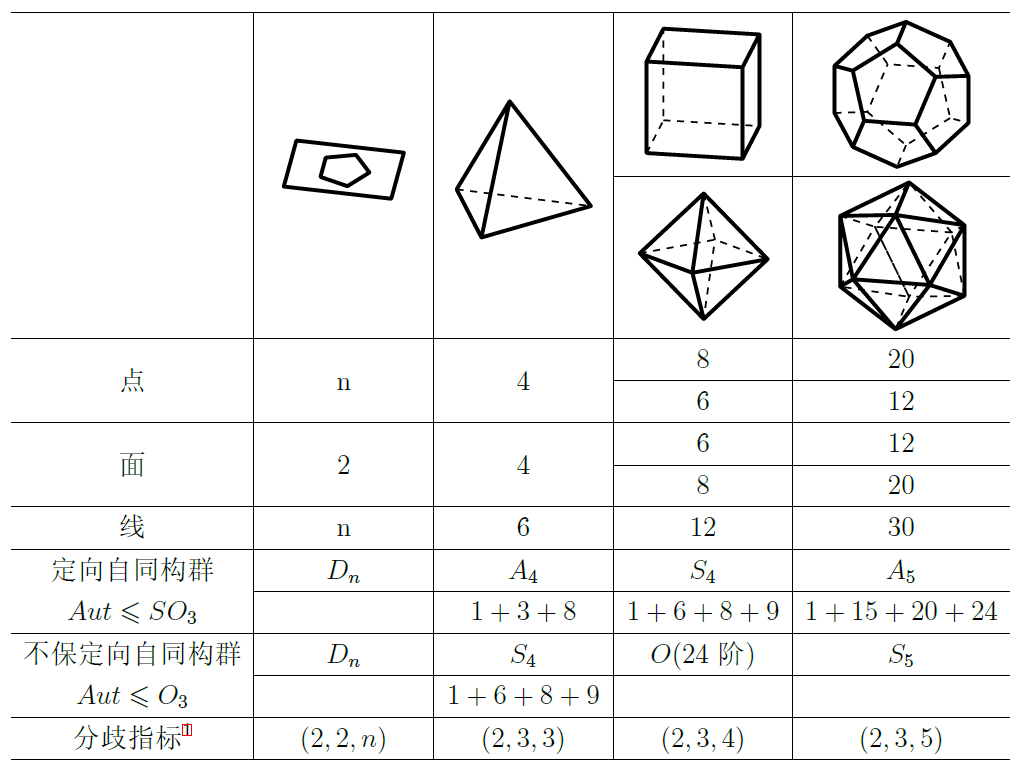
\includegraphics[width=0.98\textwidth]{snip/propofpoly.png}
\end{table}

	正多面体的重要性在于对称性,故必然引入群的概念.将其表面投影至球面$S^2=\mathbb{P}\mathbb{C}^1$,注意到$S^2$的等距自同构群为$SO_3\cong \mathbb{P}SU_2 \cong\mathbb{R}\mathbb{P}^3$,我们有交换图表:
\begin{figure}[ht]
	\centering
	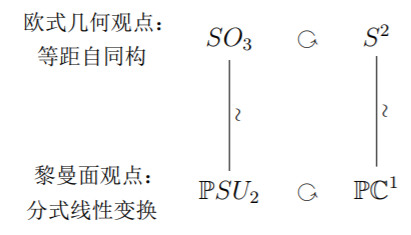
\includegraphics[]{snip/tikz-iso.png}
\end{figure}
		
		
		则正多面体的等距自同构群自然同构于$SO_3$ 的某个离散子群,记作$\Gamma$.另一方面,由\cite[5.9.1]{artin2011algebra}或\cite[2.6]{shurman1997geometry}知旋转群$SO_3$的离散子群除$\mathbb{Z}/n\mathbb{Z}$外只有上图给出的这几种;由\cite{shurman1997geometry},任一个$\Aut (\mathbb{PC}^1)$的有限子群必共轭于$SO_3$的子群,从而被清晰归类.
		

		在抽象代数中,我们已经掌握了这些群的代数性质.但现在我们再从几何/群作用的观点加深理解.
		
		\begin{enumerate}
			\item 	首先, $SO_3$的任何一个元素可以用以下方式表示:
			\begin{itemize}
				\item 	$3\times3$实矩阵;
				\item 	$2\times2$酉矩阵(作为分式线性变换)\footnote{注意$A$和$-A$表示同一个作用,我们将发展更丰富的理论来弥补这个``缺陷",如双多面体群.};
				\item 	绕某个轴旋转:\raisebox{-0.25cm}{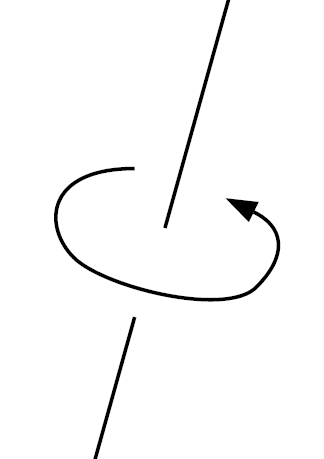
\includegraphics[width=0.5cm]{pic/rotaion.png}} (+$Id$)
			\end{itemize}
			这意味着每个$SO_3$的离散子群也可以用上述方式表示.\footnote{离散子群作为分式线性变换的表示,参见\cite[p46-47]{klein2003lectures}}.
			\item  其次, $\Gamma$在正多面体上的作用诱导了在正多面体的点、线、面上的作用.
			
			\item
			$\Gamma$ 在$S^2$上的作用,诱导了$\Gamma$ 在基本区域上的作用,这个作用是忠实且满的,即对任意基本区域$D_1,D_2$,存在唯一$\gamma\in\Gamma$使得$\gamma D_1=D_2$.所谓基本区域如下定义:
			\begin{defn}[基本区域]
				设$\Gamma$为$SO_3$的离散子群,称开集$D\subseteq S^2$为($S^2$相对于) $\Gamma$的\textbf{基本区域},如果:
				
				\begin{itemize}
					\item 对任意$\gamma\in\Gamma\smallsetminus\{Id\}$, $\gamma(D)\cap D=\varnothing$;
					
					\item $S^2=\bigcup_{\gamma\in\Gamma}\overline{\gamma(D)}$.
				\end{itemize}
			\end{defn}
		容易画出$\Gamma$的基本区域,例如图\ref{pic:basicdis}的红色区域.基于对称性,往后只考虑形如右图或者其平移的基本区域. 该图形的形状规则,可以省去很多不必要的麻烦.
			\begin{figure}[ht]
					%正十二面体
					\centering
					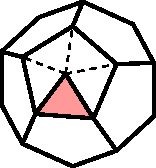
\includegraphics[]{poly/poly4-1.pdf}
					\caption{正十二面体群的基本区域}
					\label{pic:basicdis}
			\end{figure}
		\begin{exercise}
	利用基本区域计算$\Gamma$的阶. (可直接计数/求基本区域与$S^2$的面积比)
\end{exercise}

\item  既然群$\Gamma$作用于集合$S^2$,我们有轨道集$S^2/\Gamma$.在拓扑上,由右图可以看出$S^2/\Gamma\overset{\sim}{\longrightarrow}S^2$.
以Riemann曲面的观点,在赋予$S^2/\Gamma$标准的复结构之后,商映射$S^2\xtwoheadrightarrow{} S^2/\Gamma$可视作Riemann曲面之间的分歧覆叠
$$\varPhi:\mathbb{PC}^1\xtwoheadrightarrow{}\mathbb{PC}^1/\Gamma\overset{\sim}{\longrightarrow}\mathbb{PC}^1$$
该映射可视作$\mathbb{C}$上的有理函数\footnote{这些有理函数均可计算,见表\ref{tb:equations}}.
\begin{figure}[ht]
	
	\begin{minipage}[t]{.34\textwidth}
		\vspace{0.1cm}
		%正十二面体
		\centering
		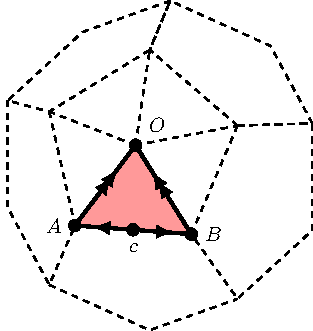
\includegraphics[width=3cm]{poly/poly4-2.pdf}
		
	\end{minipage}
	\begin{minipage}[t]{.64\textwidth}
		\vspace{0.1cm}
		\centering
		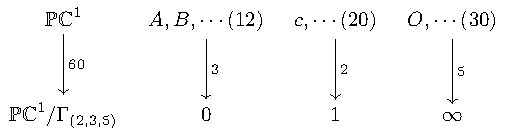
\includegraphics[]{commu/commu2.pdf}
		\caption*{在$0,1,\infty$处分歧,分歧指标为$(2,3,5)$}
	\end{minipage}
	\caption{例:正十二面体}
	\label{pic:comm2}
\end{figure}

\begin{exercise}
	写出(或画出)以上分歧覆叠的分歧点与对应的分歧指标,如图\ref{pic:comm2}.
\end{exercise}

为方便起见,我们用分歧指标作为下标来标记正多面体的定向自同构群,如$\Gamma_{(2,3,5)}$为正十二面体的定向自同构群.\footnote{该群作为$SO_3$的子群,依赖于正多面体在空间中的摆放位置,习惯上固定了正多面体的位置.}
\end{enumerate}


这些多面体之间同样有趣味的关系:
\begin{figure}[ht]
		\begin{minipage}[t]{.28\textwidth}
		\centering
		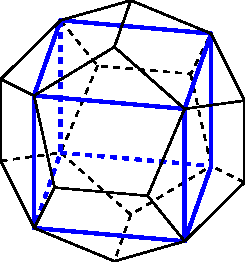
\includegraphics[scale=0.8]{poly/poly24.pdf}
		\caption{}
		\label{eg:fig1}
	\end{minipage}
	\begin{minipage}[t]{.22\textwidth}
		\centering
		%正方体套三角锥
		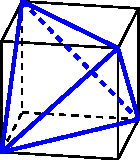
\includegraphics[]{poly/poly12.pdf}
		\caption{}
		\label{eg:fig2}
	\end{minipage}
	\begin{minipage}[t]{.22\textwidth}
		\centering
		%正方体套对角线
		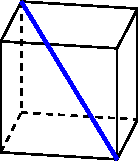
\includegraphics[]{poly/poly001.pdf}
		\caption{}
		\label{eg:fig3}
	\end{minipage}
	\begin{minipage}[t]{.22\textwidth}
		\centering
		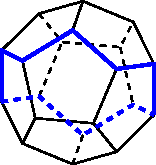
\includegraphics[]{poly/poly04.pdf}
		\caption{}
		\label{eg:fig4}
	\end{minipage}
\end{figure}

\begin{example1}\
		\begin{itemize}
			\item 图\ref{eg:fig1}给出$\Gamma_{(2,3,5)}$的一个12阶子群$A_4$;
			
			\item 不同的正方体给出不同且互相共轭的12阶子群;
			
			\item $\Gamma_{(2,3,5)}$中的元素给出5个正方体的置换,即群同态$\alpha:\Gamma_{(2,3,5)}\longrightarrow S_5$.易验证$\ker(\alpha)=\{Id\}$, $Im(\alpha)=A_5$.因此$\Gamma_{(2,3,5)}\cong A_5$.
			
		\end{itemize}
	
\end{example1}
\begin{example1}
		同上,图\ref{eg:fig2}给出$\Gamma_{(2,3,4)}$的6阶子群$A_4$及群同态$\Gamma_{(2,3,4)}\longrightarrow S_2$.
\end{example1}
\begin{example1}		
		同上,图\ref{eg:fig3}给出$\Gamma_{(2,3,4)}$的4个互相共轭的6阶子群$D_3$及群同态$\Gamma_{(2,3,4)}\longrightarrow S_4$.由此可得$\Gamma_{(2,3,4)}\cong S_4$.
\end{example1}
\begin{example1}
		同上,图\ref{eg:fig4}给出$\Gamma_{(2,3,5)}$的6个互相共轭的10阶子群$D_5$及群同态$\Gamma_{(2,3,5)}\longrightarrow S_5$.由此可得$\Gamma_{(2,3,5)}\cong S_5$.
\end{example1}


\begin{exercise}
	写出(或画出)以上分歧覆叠的分歧点与对应的分歧指数.这些分歧覆叠均可视作有理函数且可计算,可查阅表\ref{tb:equations}.
\end{exercise}

从态射的角度,对$\Aut (\mathbb{P}\mathbb{C}^1)$的两个离散子群$H \subseteq G$,我们能得到分歧覆叠$\mathbb{P}\mathbb{C}^1/H \xtwoheadrightarrow{} \mathbb{P}\mathbb{C}^1/G$.我们可以画出/写出分歧点与对应的分歧指标,给出该覆叠所对应的有理函数.\footnote{部分覆叠所对应的有理函数,见表2.在第\ref{sec:inverse-alge}节我们会使用更方便的方法来计算这些有理函数.}

作为抽象理论的补充,我们以一个具体的例子来结束本小结.

\begin{exercise}
	给定群嵌入$\Gamma_{(2,3,3)}\xhookrightarrow{\quad}\Gamma_{(2,3,5)}$,尝试计算分歧覆叠$\mathbb{PC}^1/\Gamma_{(2,3,3)}\xtwoheadrightarrow{}\mathbb{PC}^1/\Gamma_{(2,3,5)}$ 的信息.
\end{exercise}
\begin{proof}
	为方便起见,调整$\mathbb{PC}^1/\Gamma_{(2,3,3)}$的基本区域为一个五边形,如图\ref{fig:tran}.通过对图\ref{fig:tran}的观察,得到分歧指标如图
	\ref{fig:ramify1}.
	
	
	
	\begin{figure}[ht]
		\begin{minipage}[t]{.25\textwidth}
			\vspace{0cm}
			\centering
			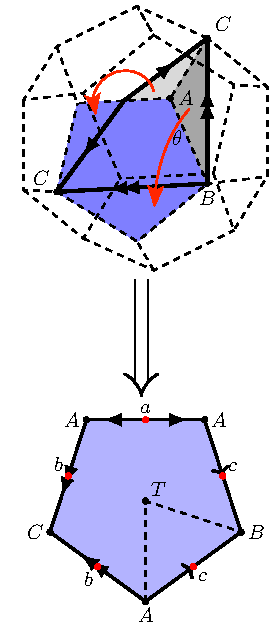
\includegraphics[width=3cm]{planet/planet5.pdf}
			\caption{}
			\label{fig:tran}
		\end{minipage}
		\begin{minipage}[t]{.65\textwidth}
			\vspace{0cm}
			\centering
			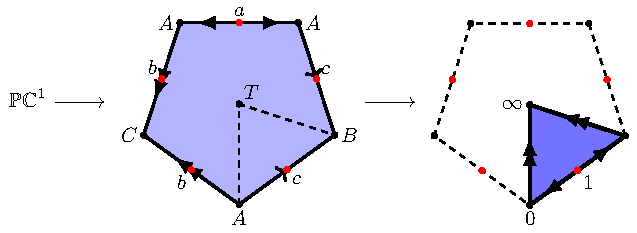
\includegraphics[width=9cm]{planet/planet3.pdf}
			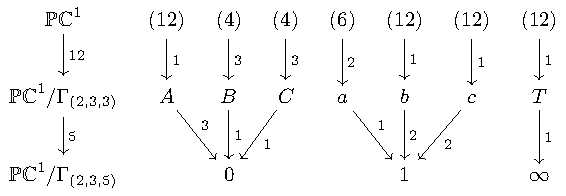
\includegraphics[]{commu/commu1.pdf}
			\caption{分歧点与分歧指标}
			\label{fig:ramify1}
		\end{minipage}
		
	\end{figure}
	
	
	
	
	
	现在我们来求该覆叠所对应的有理函数$Z(r)$.
	
	取
	$$\gamma:\mathbb{PC}^1/\Gamma_{(2,3,3)}\overset{\sim}{\longrightarrow}\mathbb{PC}^1\qquad T\longmapsto\infty,\;a\longmapsto0,\;A\longmapsto\alpha$$ 其中$\alpha\in\mathbb{R}\smallsetminus\{0\}$为待定参数.
	\begin{itemize}
		\item 由Schwarz反射原理, $\gamma(B)=\overline{\gamma(C)}:=z_0$, $\gamma(b)=\overline{\gamma(c)}$.
		\item $Z(r)$为5次多项式, $Z(0)=1,Z(\alpha)=Z(z_0)=Z(\overline{z_0})=0$.
		
		\item $Z(r)=c(r-\alpha)^3(r^2-\beta r+\gamma),\quad\beta,\gamma\in\mathbb{R}$.这蕴含$c=-\frac{1}{\alpha^3\gamma}\in\mathbb{R} \smallsetminus \{0\}$.
	\end{itemize}
	
	调节$\alpha$使得$c=-1/1728$\footnote{取$\alpha=1$后得到$c$的值,重新取$\alpha=-(1728c)^{\frac{1}{5}}$即可.},则
	$$Z:Z-1:1\;=\;(r-\alpha)^3(r^2-\beta r+\gamma):r(r^2-\epsilon r+\xi)^2:-1728,$$
	其中$\alpha,\beta,\gamma,\epsilon,\xi\in\mathbb{R}$.上式蕴含
	\begin{equation}
	(r\alpha)^3(r^2-\beta r+\gamma)+1728=r(r^2-\epsilon r+\xi)^2.
	\end{equation}
	
	对比$r$的次数展开后,这个方程组有$5$个变量, $5$个方程,看似已无解.但是,所谓“山重水复疑无路,柳暗花明又一村”,在\textbf{奇妙}的消元法之后,我们得到
	\[Z:Z-1:1\;=\;(r-3)^3(r^2-11r+64):r(r^2-10r+45)^2:-1728.\]
	
	下面简要陈述这个奇妙的消元法,摘自\cite[P111]{klein2003lectures}.
	
	在(0.1)式两边求导,得到
	$$(r-\alpha)^2\big(5r^2-(2\alpha+4\beta)r+(\alpha\beta+3\gamma)\big)=(r^2-\epsilon r+\xi)(5r^2-3\epsilon r+\xi). $$
	但由于$b,c\neq a$,故$(r-\alpha)$与$(r^2-\epsilon r+\xi)$互素,故有方程组
	$$\begin{cases}5\epsilon=2\alpha+4\beta\\5\xi=\alpha\beta+3\gamma\\10\alpha=3\epsilon\\5\alpha^2=\xi\end{cases}$$
	依次消去$\epsilon,\xi,\beta$得到$64a^2=9\gamma$;对(0.1)式取$r=0$得$\alpha^3\gamma=1728$.综合两式,我们有$a^5=3^5$,由$a\in\mathbb{R}$知$a=3$.其余参数均容易顺次求出.
	\begin{exercise}\label{exercise:function}
		利用分歧映射以及上文给出的映射$\gamma$,说明覆叠$\mathbb{P}\mathbb{C}^1 \longrightarrow \mathbb{P}\mathbb{C}^1/\Gamma_{(2,3,3)}$所对应的有理函数$r(z)$可记为$\frac{t^2(z)}{f(z)}$,其中$t(z)$为6次多项式,在立方体的面心各有一个1阶零点; $f(z)$为12次多项式,于正十二面体的面心处各有一个1阶零点.
	\end{exercise}
	
\end{proof}
\section{综述}
上一节中,我们从正多面体的对称性出发,导出分歧覆叠
$$\varPhi\colon \mathbb{PC}^1 \xrightarrow{\qquad} \mathbb{PC}^1/\Gamma \cong \mathbb{PC}^1$$
%数学中对逆映射特别在意,在这里也是:
%\begin{center}
%	\fbox
%	{给定$Z \in \mathbb{C}$,尝试赋予$\varPhi^{-1}(Z)$恰当的定义,并描述$\varPhi^{-1}(Z)$的性质.}
%\end{center}
在第\ref{sec:inva}节,我们将利用不变量理论给出$\Phi$的表达式.在第\ref{sec:inverse-comp},\ref{sec:inverse-alge}节,我们将以复分析/近世代数的方式研究$\Phi^{-1}$.在最后,我们将研究如何用模形式/正十二面体方程来解一般的五次方程. 整个流程图如下:
\begin{figure}[ht]
	
	\begin{minipage}[t]{.9\textwidth}
		\vspace{0.1cm}
		\centering
		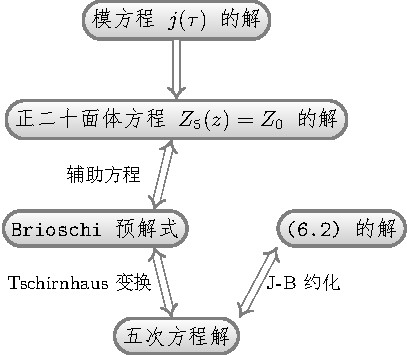
\includegraphics{Flowchart/Mainflowchart.pdf}
		
	\end{minipage}
	\label{pic:flow}
\end{figure}
\section[不变量理论]{不变量理论\protect\footnote{本节主要参考了\cite[Chapter 3]{shurman1997geometry}.}}\label{sec:inva}

	在本节中,记$\mathbb{C}_n\homopoly$为$n$次齐次多项式构成的集合, $\mathbb{C}\homopoly:= \bigcup_{n=0}^{+\infty} \mathbb{C}_n\homopoly$为齐次多项式构成的集合,注意$\mathbb{C}_n[z_1,z_2]$与$\mathbb{C}_n\homopoly$的区别.记$f\sim g \Leftrightarrow $存在$k \in \mathbb{C}^*$, $f=kg$.习惯性称齐次多项式为形式(form)\footnote{这是因为$n$次齐次多项式可视作$\mathcal{O}_{\mathbb{PC}^1}(n)$的一个全纯截影.}. 

\subsection{不变函数与半不变量}
函数空间(层)是几何对象的灵魂.直觉来看, $X/G$上的函数可视为$X$上满足对称性($f(\gamma z)= f(z)$)的函数\footnote{然而这不是常态. $X/G$可能是很怪异的空间(如$\mathbb{P}^2/PGL_2$,见\cite[Example 10.8]{mumford1995algebraic}),函数空间的选取也需要足够合适.但对于有限群在代数簇上的作用,商空间总是存在并构成一个代数簇,见\cite{mumford1995algebraic}.},这使得不变量理论进入了我们的视野:
\begin{defn}
	设有限群$\Gamma$作用在$\mathbb{PC}^1$上.称亚纯函数$f$为$\Gamma$-\textbf{不变函数},若对任意$\gamma \in \Gamma, z \in \mathbb{PC}^1$,
	$$f(\gamma z)=f(z)$$
\end{defn}
在黎曼面课上我们知道,任一个$\mathbb{PC}^1$上的亚纯函数$f$可视作两个互质多项式$G,H\in \mathbb{C}\homopoly$的比\footnote{今后均假设$G,H$互质.}:
$$f\big(\homopoly\big)=\big[G(z_1,z_2):H(z_1,z_2)\big], \quad\text{ 简记为 } \,f=[G:H]$$
这使我们想要探索$\Gamma$与$\mathbb{C}\homopoly$的关系.定义
$$\Gamma':= \left\{ A \in SU_2 \mid \bar{A} \in \Gamma \right\}$$
为群$\Gamma$的提升,则
\begin{itemize}
	\item $\Gamma' \subseteq SU_2$作用在$\mathbb{C}\homopoly$上$\left( \begin{bmatrix}
	a & b \\ c & d
	\end{bmatrix} (z_1,z_2):= (az_1+bz_2:cz_1+dz_2) \right)$
	\item $|\Gamma'|=2|\Gamma|$, $\Gamma$为有限群;
	\item 记$\gamma' \in \Gamma'$为$\gamma \in \Gamma$的提升,则
	$$f \circ \gamma = [G \circ \gamma' : H \circ \gamma']$$
\end{itemize}
\begin{defn}
	称形式$F$以$\bigchi_F: \Gamma' \longrightarrow \mathbb{C}^*$为特征的$\Gamma'$-\textbf{半不变量},若对任意$\gamma' \in \Gamma'$,
	$$F\big(\gamma' \homopoly\big)=\bigchi_F(\gamma')\, F\big(\homopoly\big),\quad \text{ 简记为 } \,F \circ \gamma'= \bigchi_F(\gamma') F. $$
	当$\bigchi_F$平凡时,我们称形式$F$为$\Gamma$-不变量.
\end{defn}
容易看出,若$G,H \in \mathbb{C}_n\homopoly$均为以$\bigchi$为特征的$\Gamma'$-半不变量,则$f=[G:H]$为$\Gamma$-不变函数.令人惊奇的是,反之也是成立的:
\begin{theorem}[{\cite[Proposition 3.1.2]{shurman1997geometry}}]\label{thm:repofinvfunc}
	设亚纯函数$f=[G:H]$为$\Gamma$-不变函数,则存在特征$\bigchi \in \Hom_{Grp}(\Gamma', \mathbb{C}^*)$,使得$G,H$为以$\bigchi$为特征的$\Gamma'$-半不变量.
\end{theorem}
\begin{proof}
	直接的代数论证,见\cite[exercise 3.13]{shurman1997geometry}.
\end{proof}

这样我们将不变函数的问题转移到$\Gamma'$-半不变量上.我们将刻画所有的不变量,以及描述其中特殊元素之间的关系,从而得到它们的表达式.可以说,不变量理论是定量计算的有力武器.
\subsection{轨道形式}
我们知道, $\mathbb{PC}^1$上的全纯截影由其除子(记录截影零点的位置和阶数)唯一决定(忽略常数因子).记$\divi(f)=\sum_{\text{finite}}n_iP_i$,则$\divi(f\circ \gamma')=\sum_{\text{finite}}n_i\gamma'(P_i)$,故
\begin{equation*}
\begin{aligned}
&f\text{ 为 }\,\Gamma'\text{-半不变量}\\
\Leftrightarrow\,&\text{对任意}\,\gamma' \in \Gamma',\, \divi(f)=\divi(f \circ \gamma')\\
\Leftrightarrow\,& \divi(f)=\sum_{\text{i finite}} \sum_{P \in \mathcal{O}_i}P,\,\text{其中$\mathcal{O}_i$为$\Gamma$在$\mathbb{PC}^1$上的某个轨道.}\\
\end{aligned}
\end{equation*}
故$\Gamma'$-半不变量亦可被称作轨道形式(orbit form).

我们定义一类特殊的轨道形式,这类轨道形式可以有清晰的表达,并且具有相同的特征.回忆定理 \ref{thm:repofinvfunc},这给出了我们需要的$\Gamma$-不变函数.
\begin{defn}[全轨道形式]
	我们称$f \in \mathbb{C}_{|\Gamma|}\homopoly$为\textbf{全轨道形式},若存在轨道$\mathcal{O}_f$,使得
	$$\divi (f)= \frac{|\Gamma|}{|\mathcal{O}_f|} \sum_{P \in \mathcal{O}_f}P$$
\end{defn}

设$F_p$为以$p=[p_1,p_2]$为零点的全轨道形式,对每个$\gamma \in \Gamma$写成两个线性映射的商: $\gamma=\frac{\gamma_1}{\gamma_2}$,则
$$F_p(z_1,z_2) \sim \prod_{\gamma \in \Gamma}\left(\gamma_2(p_1,p_2)z_1-\gamma_1(p_1,p_2)z_2\right)$$
可以看出,固定$\gamma_0 \in \Gamma$, $\bigchi_{F_p}(\gamma_0)$是关于$p$良定义的连续函数,而$|\Gamma|$次单位根是离散空间,故$\bigchi_{F_p}(\gamma_0)$为常值函数,所有全轨道形式具有相同的特征,记为$\bigchi_{\Gamma}$.

对正多面体群\footnote{旋转群只在两个轨道处退化,这时理论只需略微修正,如令$F_3=z_1^n-z_2^n$.},全轨道形式恰好在三个轨道处(记为$\mathcal{O}_1,\mathcal{O}_2,\mathcal{O}_3$)退化\footnote{指$|\Gamma| \neq |\mathcal{O}_i|$.},成为某个非退化轨道形式的$v_i:=|\Gamma|/|\mathcal{O}_i|$次幂.我们写出这些非退化轨道形式:
$$F_i= \prod_{[p_1:p_2] \in \mathcal{O}_i}(p_2z_1-p_1z_2)$$
记所对应的特征为$\bigchi_i$.
\begin{example1}
	对旋转群$\Gamma=\mathbb{Z}/n\mathbb{Z} \curvearrowright \mathbb{PC}^1$,此时只有2个非平凡轨道:
	$$\mathcal{O}_1=\left\{[1:0] \right\} \qquad \mathcal{O}_2=\left\{[0:1] \right\}$$
	故$F_1=z_2$, $F_2=z_1$.(不在意常系数).对$s_{n}':=\begin{pmatrix}
	\omega_{2n} & 0 \\ 0 & \bar{\omega}_{2n}
	\end{pmatrix} \in \Gamma'$, 
	$$F_1 \circ \homopoly =F_1[\omega_{2n}z_1 : \bar{\omega}_{2n} z_2] = \bar{\omega}_{2n} z_2=\bar{\omega}_{2n} F_1$$
	故$$\bigchi_1:s_n' \longmapsto \bar{\omega}_{2n}, \quad -I \longmapsto -1. $$
	同理可证$\bigchi_2=\bar{\bigchi}_1$.当取$F_3=z_1^n-z_2^n$时, $\bigchi_3=\bigchi_{\Gamma}=\bigchi_1^n$.
\end{example1}
\begin{example1}
	对正二面体群$\Gamma=D_{n} \curvearrowright \mathbb{PC}^1$,此时三个轨道分别为
	\begin{equation*}
	\mathcal{O}_1=\left\{ [1:0], [0,1] \right\}, \quad
	\mathcal{O}_2=\left\{ [\omega_{n}^a:1] \big| a \in \mathbb{Z} \right\}, \quad
	\mathcal{O}_3=\left\{ [\omega_{2n}\omega_{n}^a:1] \big| a \in \mathbb{Z} \right\} .
	\end{equation*}
	得到三个半不变量
	$$F_1=z_1z_2, \quad F_2=\frac{z_1^n-z_2^n}{2}, \quad F_3=\frac{z_1^n+z_2^n}{2}. $$
	记$s_{n}':=\begin{pmatrix}
	\omega_{2n} & 0 \\ 0 & \bar{\omega}_{2n}
	\end{pmatrix}$, $t':=\begin{pmatrix}
	0 & i \\ i & 0
	\end{pmatrix} \in \Gamma'$, 通过计算得到
	\begin{equation*}
	\begin{aligned}
	&\bigchi_1:s_n' \longmapsto \phantom{-}1, \quad t' \longmapsto -1\\
	&\bigchi_2:s_n' \longmapsto -1, \quad t' \longmapsto i^n \qquad \bigchi_3=\bar{\bigchi}_2
	\end{aligned}
	\end{equation*}
\end{example1}
下面这个定理告诉我们,这些特殊的轨道形式给出了所有(全)轨道形式的表达:(特殊蕴含一般)
\begin{theorem}[{\cite[Theorem 3.3.2, Exercise 3.2.3]{shurman1997geometry}}]\label{thm:expr} 任一个全轨道形式均可以表达为$F=\lambda_1F_1^{v_1}+\lambda_2F_2^{v_2}$, $\lambda=[\lambda_1,\lambda_2] \in \mathbb{PC}^1$的形式.
	
	任一个轨道形式均可以表达为
	$$F=F_1^{e_1}F_2^{e_2}F_3^{e_3}\prod_{\substack{\lambda=[\lambda_1:\lambda_2]\\\text{finite}}}(\lambda_1F_1^{v_1}+\lambda_2F_2^{v_2})^{e_{\lambda}},\qquad 0 \leqslant e_i < v_i$$
	的形式.
	
	这些表达在忽略常系数的情况下唯一.
\end{theorem}
\begin{proof}
	只需观察(全)轨道形式的零点位置即可.
\end{proof}
\begin{corollary}
	$F_1,F_2,F_3$之间存在唯一的代数关系:
	$$c_1F_1^{v_1}-c_2F_2^{v_2}+c_3F_3^{v_3}=0$$
\end{corollary}
这时已可以用暴力列举法来算$F_i$了,但计算仍然繁杂.通过协变函子的帮助,可以由$F_1$推出$F_2$和$F_3$.在此之前,我们以正二十面体的$F_1$的计算为例,来说明$F_1$的计算方式.
\begin{example1}[正二十面体的$F_1$]
	写出正十二面体的面点(即是正二十面体的顶点)对应的轨道
	$$\mathcal{O}_1:=\left\{0,\infty,\omega_5^i\varphi,-\omega_5^i\varphi^{-1} \right\}$$
	得到
	\begin{equation*}
	\begin{aligned}
	F_1 = \,& z_1z_2 \prod_{i=0}^{4}(z_1-\omega_5^i\varphi z_2) \prod_{i=0}^{4}(z_1+\omega_5^i\varphi^{-1} z_2) \\
	= \,& z_1z_2(z_1^5-\varphi^5 z_2^5)(z_1^5+\varphi^{-5}z_2^5)\\
	= \,& z_1z_2(z_1^{10}-(\varphi^5-\varphi^{-5})z_1^5z_2^5-z_2^{10})\\
	= \,& z_1z_2(z_1^{10}+11z_1^5z_2^5-z_2^{10})\\
	\end{aligned}
	\end{equation*}
	由于$A_5$是非交换单群,故无非平凡1维表示.
\end{example1}
\subsection{协变函子$H$, $J$}
\begin{defn}
	我们称协变函子$C: \mathbb{C} \homopoly \longrightarrow \mathbb{C} \homopoly$与$\Gamma'$相容,若存在$e\in \mathbb{Z}$,使得对任意$\gamma' \in \Gamma'$, $a \in \mathbb{C}^*$, $F \in \mathbb{C} \homopoly$,有
	$$C(F \circ \gamma')= C(F) \circ \gamma' \qquad C(aF)=a^eC(F)$$
	当$F$为以$\bigchi_F$为特征的$\Gamma'$-不变量时, $C(F)$为以$\bigchi_F^e$为特征的$\Gamma'$-不变量.
\end{defn}
\begin{example1}
	对$\Gamma'$-不变量,定义Hesse函子$H$与Jacobi函子$J$:
	$$M_H(F)= \begin{bmatrix}
	D_{11}F & D_{12}F \\ D_{21}F & D_{22}F 
	\end{bmatrix} 	\qquad H=\det M_H$$
	$$M_J(F)= \begin{bmatrix}
	D_{1}F & D_{1}HF \\D_{2}F & D_{2}HF
	\end{bmatrix} 	\qquad J=\det M_J$$
	经过繁复的计算, $H$, $J$均与$\Gamma'$相容,并且
	$$\deg (HF)=2(\deg F-2), \quad \deg(JF)=3(\deg F-2),$$
	$$ \quad \bigchi_{HF}=\bigchi_F^2, \quad \bigchi_{JF}=\bigchi_F^3. $$
\end{example1}
\begin{proof}
	按顺序计算$D_i(F \circ \gamma')$, $D_{ij}(F \circ \gamma')$, $H(F \circ \gamma')$, $J(F \circ \gamma')$:
	
	\begin{flalign*}
	D_i(F \circ \gamma') = & D_i\big(F(a_{11}z_1+a_{12}z_2,a_{21}z_1+a_{22}z_2) \big)&\\                                                                 
	= & \sum_{k \in \{1,2\}} a_{ki} (D_kF) \circ \gamma'\footnotemark &
	\end{flalign*}
	\footnotetext{矩阵表示可以让我们对今后的计算看得更清楚:
		$$\begin{bmatrix}
		D_1(F \circ \gamma') \\ D_2(F \circ \gamma')
		\end{bmatrix}=
		\begin{bmatrix}
		a_{11} & a_{21} \\ a_{12} & a_{22}
		\end{bmatrix}
		\begin{bmatrix}
		D_1F \circ \gamma' \\ D_2F \circ \gamma'
		\end{bmatrix}
		$$}
	\begin{flalign*}
	D_{ij}(F \circ \gamma') = &	D_i \big[D_j (F \circ \gamma') \big]				&\\
	= &	D_i\left[\sum_{l}a_{lj}(D_lF) \circ \gamma' \right]						&\\
	= &\sum_{l}a_{lj}D_i \big[(D_lF) \circ \gamma'\big]							&\\
	= &	\sum_{l}a_{lj}\left[\sum_k a_{ki} (D_kD_lF) \circ \gamma'\right]						&\\
	= &	\sum_{k,l} a_{ki} (D_{kl}F) \circ \gamma' a_{lj}						&
	\end{flalign*}
	\begin{flalign*}
	H(F \circ \gamma')= &	\det \begin{bmatrix}
	D_{11}(F \circ \gamma') & D_{12}(F \circ \gamma') \\
	D_{12}(F \circ \gamma') & D_{22}(F \circ \gamma')
	\end{bmatrix}						&\\	
	= &	\det \left( \begin{bmatrix}
	a_{11} & a_{21} \\ a_{12} & a_{22}
	\end{bmatrix}
	\begin{bmatrix}
	(D_{11}F) \circ \gamma' & (D_{12}F) \circ \gamma' \\
	(D_{21}F) \circ \gamma' & (D_{22}F) \circ \gamma'
	\end{bmatrix}
	\begin{bmatrix}
	a_{11} & a_{12} \\ a_{21} & a_{22}
	\end{bmatrix}\right)						&\\
	= &	\det \begin{bmatrix}
	(D_{11}F) \circ \gamma' & (D_{12}F) \circ \gamma' \\
	(D_{21}F) \circ \gamma' & (D_{22}F) \circ \gamma'
	\end{bmatrix}						&\\
	= &	H(F) \circ \gamma'						&
	\end{flalign*}
	\begin{flalign*}	
	J(F \circ \gamma')	= &	\det	\begin{bmatrix}
	D_1(F \circ \gamma') & D_1H(F \circ \gamma') \\
	D_2(F \circ \gamma') & D_2H(F \circ \gamma')
	\end{bmatrix}					&\\	
	= &	\det \begin{bmatrix}
	D_1(F \circ \gamma') & D_1(HF \circ \gamma') \\
	D_2(F \circ \gamma') & D_2(HF \circ \gamma')
	\end{bmatrix}						&\\
	= &	\det \left( \begin{bmatrix}
	a_{11} & a_{21} \\ a_{12} & a_{22}
	\end{bmatrix}
	\begin{bmatrix}
	(D_{1}F)\circ \gamma' & (D_{1}HF)\circ \gamma' \\
	(D_{2}F)\circ \gamma' & (D_{2}HF)\circ \gamma'
	\end{bmatrix}
	\right)						&\\
	= &	(JF) \circ \gamma'						&	
	\end{flalign*}
	其余论断均显然.
\end{proof}

通过对次数的比照,运用定理\ref{thm:expr},以及一点额外的计算,我们惊奇地发现\footnote{我怀疑这里可以用$H$, $J$的几何直观看出,但我没有证据.},对非退化的正多面体群(亦即,除$C_n$, $D_n$外), $F_2=H(F_1)$, $F_3=J(F_1)$.这样我们得到了所有有限群对应的$F_1,F_2,F_3$以及之间的代数关系,如图\ref{tb:equations}.可以说,到目前为止,我们对$\mathbb{PC}^1$上的不变量理论有了一个较为彻底的理解.
\subsection{结论汇总}
	\begin{table}[ht]
		\centering
		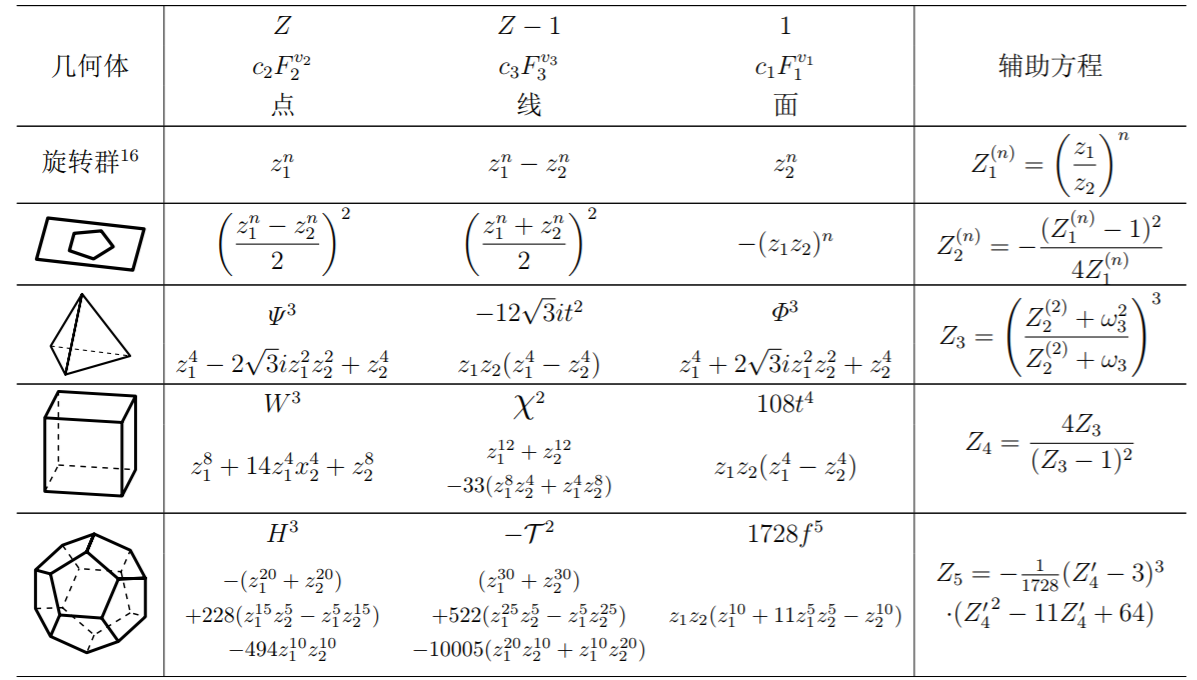
\includegraphics[width=0.98\textwidth]{snip/eqpoly.png}
	\caption{正多面体对应方程}
	\label{tb:equations}
\end{table}
\footnotetext{$Z_1^{(n)}$不对应几何体, $v_1 \neq 2$ !}

\begin{remarks}\
	\begin{enumerate}[1.]
		\item 由于嵌入正十二面体的立方体为倾斜放置,辅助方程为$Z_4'$,与$Z_4$相差一个分式线性变换.倾斜的立方体对应的$F_1,F_2,F_3$及其代数关系如下:
	\begin{figure}[ht]
	\centering
	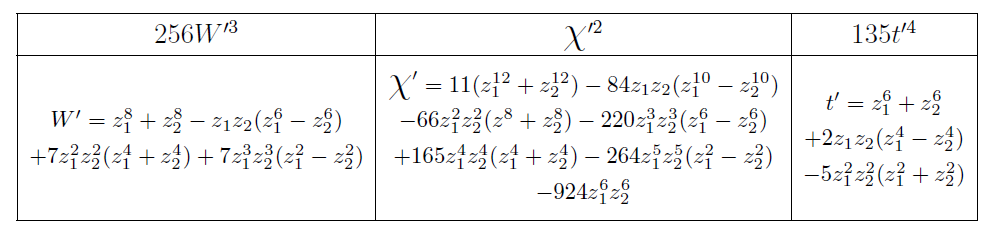
\includegraphics[width=0.98\textwidth]{snip/slantpoly.png}
\end{figure}
		\item 通过辅助方程,除$Z_5(z)$以外的其他方程均可解出,且为根式解.但是正十二面体所对应的最后一个辅助方程是5次方程,运用Galois的理论我们得到该方程的不可解性.我们将在第\ref{sec:inverse-alge}节中具体解释该现象.
	\end{enumerate}
\end{remarks}
返回看我们最初的问题,我们可以轻而易举地写出一个非常值的$\Gamma$-不变函数:
$$Z:= \frac{c_2F_2^{v_2}}{c_1F_1^{v_1}}$$
这可看作是黎曼面$\mathbb{PC}^1/\Gamma$上的一个亚纯函数,由于$\mathbb{PC}^1/\Gamma \cong \mathbb{PC}^1$,故$\mathbb{PC}^1/\Gamma$上的亚纯函数空间是$\mathbb{C}(Z) = \mathbb{C}(z)^{\Gamma}$.从代数的角度,这个等式可以从对例外轨道形式的描述中得到,详见\cite[3.5,3.6]{shurman1997geometry}.
\begin{remarks}\
	\begin{enumerate}
		\item 如何定义商空间$\mathbb{PC}^1/\Gamma$的代数簇结构?这里我们讨论的是$\Gamma'$-半不变量,当考虑对应的$\Gamma’$-不变量(平凡特征)时,不变量代数$\mathbb{C}[z_1,z_2]^{\Gamma'}$所对应的射影概型$\Proj\mathbb{C}[z_1,z_2]^{\Gamma'}$即为所求的商空间.注意这里作为代数簇, $$\Proj\mathbb{C}[z_1,z_2]^{\Gamma'} = \mathbb{PC}^1//\Gamma \neq \mathbb{PC}^1.$$
		\item  有了坐标环,我们可以发掘新的理论: $\mathbb{C}[z_1,z_2]^{\Gamma'}$同构于$\mathbb{C}[f_1,f_2,f_3]/(F(f_1,f_2,f_3))$的形式,商空间反射锥所对应的唯一奇点$(0,0,0)$上记录着群$\Gamma'$的信息,另外,反射锥在奇点消解过后得到的例外除子对应的对偶图和$\Gamma$的不可约表示导出的McKay图是同一个Dynkin图,详情可见\cite{han2018Mckay}.
		\item 半不变量可视为`` $\mathbb{PC}/\Gamma$上权为$n$的模形式",反过来,模形式也可视为某种形式的半不变量,对应的是同余子群$\Gamma$的二维特征.
	\end{enumerate}
	
\end{remarks}
\section{多值函数:复分析视角}\label{sec:inverse-comp}


按照复分析观点, $\varPhi^{-1}(Z)$不过是一个多值函数.那么自然的流程如下:
\begin{itemize}
	\item 找出多值函数合适的支点和支线;
	\item 找出其单值解析分支并表达(Schwartzian $s$-function;在支点处的Laurent展开);
	\item 寻求不同单值解析分支之间的关系(支点附近, deck变换);
	\item 找出单值解析分支满足的常微分方程.
\end{itemize}
由于我们选取的$\varPhi$只在$0,1,\infty$处分歧,取过这三个点的直线$\mathbb{R} \cup \{\infty\}$, $\varPhi\left(\mathbb{R} \cup \{\infty\}\right)$将原空间划分为一个个三角形,每个三角形通过$\varPhi$同上/下半平面双全纯等价.这样,取2个相邻的三角形即构成$\varPhi$的单值解析分支.
\begin{remark}
	给定双全纯映射
	\begin{figure}[ht]
		\begin{minipage}[t]{.9\textwidth}
			\vspace{0.1cm}
			\centering
			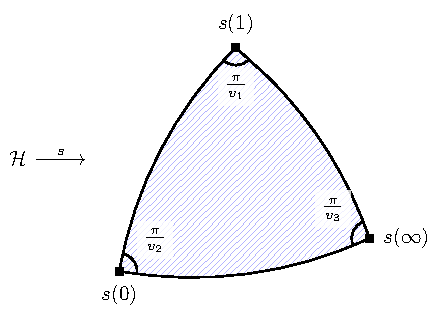
\includegraphics{pic/halfspace5.pdf}
		\end{minipage}
		\label{pic:Htriangle}
	\end{figure}
	
	通过Schwarz反射得到多值函数
	\begin{figure}[ht]
			\centering
			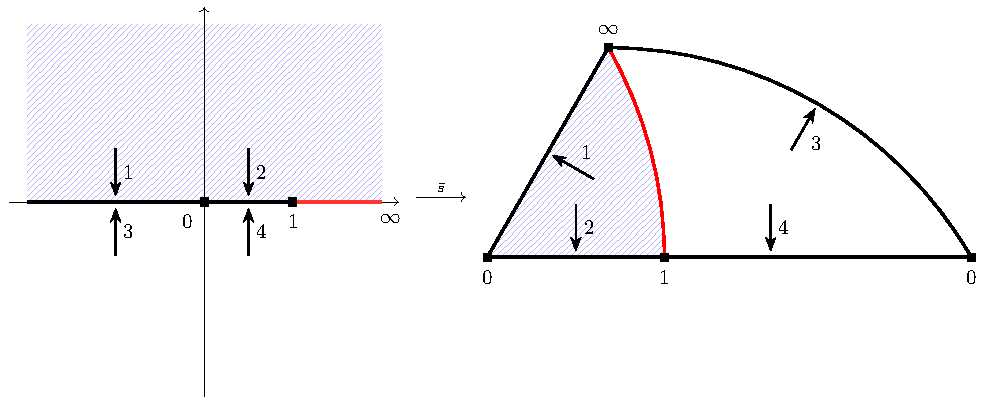
\includegraphics[width=.98\textwidth]{pic/halfspace4.pdf}
		\label{pic:Ctriangle}
	\end{figure}
	称其为\textbf{Schwarz $s$-函数},记作$ s(\frac{\pi}{v_1},\frac{\pi}{v_2},\frac{\pi}{v_3},J)$.
	%其中$\mathbb{PC}^1$, $\mathbb{C}^1$, $\mathcal{H}$为唯三的单连通Riemann面.
	容易得到,当$\frac{1}{v_1}+\frac{1}{v_2}+\frac{1}{v_3}>1$时, $\bar{s}^{-1}$为有理函数$\varPhi$;当$\frac{1}{v_1}+\frac{1}{v_2}+\frac{1}{v_3}=1$时, $\bar{s}^{-1}$为特殊的双周期函数;当$\frac{1}{v_1}+\frac{1}{v_2}+\frac{1}{v_3}=1$时, $\bar{s}^{-1}$为特殊的模函数.特别地,当$(v_1,v_2,v_3)=(2,3,\infty)$时, $\bar{s}^{-1}$与$j$-函数之间只差一个分式线性变换.
	
\end{remark}
\begin{exercise}
	当$(v_1,v_2,v_3)=(\infty,\infty,\infty)$时,情况如何?
\end{exercise}

利用Schwarz-Christoffe公式\cite[p237]{ahlfors1979complex},我们得到
$$z=\varPhi^{-1}(Z)=C \int_{0}^{Z} \omega^{-\beta_2} (\omega-1)^{-\beta_3}d \omega +C', \qquad \beta_i=1-\frac{1}{v_i}=\frac{v_i-1}{v_i}$$
由于$\varPhi$在$Z_0=0,1,\infty$\footnote{对$Z_0=\infty$,形式上将$1/Z$记作$Z-Z_0$,但本质上是一样的.}点处为分歧覆叠,记分歧指数为$v$,则在其附近,有
\begin{equation}
\begin{aligned}
Z-Z_0 = & f\left((z-z_0)^v\right), 	\qquad f(0) \neq 0 \\
z-z_0 = & \alpha (Z-Z_0)^{\frac{1}{v}}+ \beta (Z-Z_0)^{\frac{1}{v}} + \gamma (Z-Z_0)^{\frac{1}{v}} + \cdots 	\qquad \alpha \neq 0   \label{eq:expansion}
\end{aligned}
\end{equation}
代入$\varPhi$即可得到$\alpha,\beta,\gamma,\cdots$.

由构造, $\Gamma$将单值解析分支映至单值解析分支,越过支线所对应的分式线性变换亦可从图中看出.

记$\eta=\eta(Z)$为其中的一个解析分支, Schwarz导数$[f]_Z=\frac{f'''}{f'}-\frac{3}{2}\left(\frac{f''}{f'}\right)^2$.由于对任意$\gamma \in SL_2(\mathbb{R})$, $[\gamma(\eta)]_Z=[\eta]_Z$,故
$$[\varPhi^{-1}]_Z:\mathbb{PC}^1 \longrightarrow \mathbb{PC}^1 \qquad Z_0 \longmapsto [\eta]_Z(Z_0)$$
为良定义的亚纯函数,故为有理函数,记为$r(Z)$.
通过对\eqref{eq:expansion}计算,得到$r(Z)$具有形式\footnote{等式 $\displaystyle[Z^{\frac{1}{v}}]_Z=\frac{1-v^2}{2v^2Z^2}$可以揭示在展开时出现的首项系数.}
$$r(Z)=\frac{v_{1}^{2}-1}{2 v_{1}^{2}(Z-1)^{2}}+\frac{A}{Z-1}+\frac{v_{2}^{2}-1}{2 v_{2}^{2} Z^{2}}+\frac{B}{Z}+C_{3}$$
再将此形式在$\infty$处Laurent展开并对比,最终得到答案
$$r(Z)=\frac{v_{1}^{2}-1}{2 v_{1}^{2}(Z-1)^{2}}+\frac{v_{2}^{2}-1}{2 v_{2}^{2}Z^2} +\frac{\frac{1}{v_{2}^{2}}+\frac{1}{v_{2}^2}-\frac{1}{v_{3}^{2}}-1}{2(Z-1) Z}$$
故我们得到了解析分支$\eta$所满足的函数方程:
$$f'''f'-\frac{3}{2} (f'')^2-r(Z)(f')^2=0$$
非线性方程比线性方程总是要复杂一些.事实上,通过计算,我们总可以将$\eta$写为某个二阶线性方程的两个解$y_1,y_2$之商.
\section{预解式:近世代数视角}\label{sec:inverse-alge}

按照近世代数观点,将$\varPhi$视作有理函数,记
$$\varPhi(z)=\frac{f(z)}{g(z)}, \qquad f,g \text{ 互素}$$
寻找$\varPhi^{-1}(Z)$亦即方程$Zg(z)-f(z)=0 \;(\text{over }\mathbb{C}(Z))$的解.那么自然的流程如下:
\begin{itemize}
	\item 给出方程所对应的Galois群.
	\item 判定该方程是否有根式解:若有,具体解出;
	\item 在给出辅助方程后尝试解出(如预解式,模函数);\footnote{这是一个递归的过程,我们也会用这些方程来尝试解其他方程(如一般的五次方程)}
\end{itemize}
在Galois理论中,我们考虑域扩张$\mathbb{C}(z)/\mathbb{C}(Z)$所对应的Galois群
$$\Gal \left(\mathbb{C}(z)/\mathbb{C}(Z)\right) \subseteq \Aut_{\mathbb{C}}(\mathbb{C}(Z)) \overset{\sim}{\longrightarrow} \PSL_2(\mathbb{C})$$
由于对$\gamma \in \Gamma$, $\gamma z \in \mathbb{C}(z)$亦为方程的一个根,故$\mathbb{C}(z)$为$\mathbb{C}(Z)$关于多项式
$$p_W(T):= Zg(T)-f(T)$$
的分裂域, $\mathbb{C}(z)/\mathbb{C}(Z)$为Galois扩张, $\Gal\left(\mathbb{C}(z)/\mathbb{C}(Z)\right) \cong \Gamma$.

另外,我们有扩张与Galois群的反向对应:
\[	\setcounter{MaxMatrixCols}{15}
\begin{array}{ccccccccc|cc}
\mathbb{C}(z) &\supseteq &\mathbb{C}(Z_1^{(2)}) &\supseteq &\mathbb{C}(Z_2^{(2)}) &\supseteq &\mathbb{C}(Z_3) &\supseteq  &\mathbb{C}(Z_4) =  \mathbb{C}(Z_4') &\supseteq  &\mathbb{C}(Z_5)\\[-0.45cm]
&\underset{2}{}&&\underset{2}{}&&\underset{3}{}&&\underset{2}{}&&\underset{5}{}&\\
\{1\} &\lhd &C_2 &\lhd &D_2  &\lhd &A_4 &\lhd &S_4 &\leqslant &S_5
\end{array}
\]
竖线左边为根式扩张与正规子群序列的对应,右边为非循环单群($\Rightarrow$不可解群)与非分式扩张的对应.

为了进一步研究$A_5$,我们引入预解式的概念,希望在给出预解式某个根后得到方程$p_W(T)=0$的根:
\begin{defn}
	我们称$r \in K$相对于Galois扩张$K/k$的\textbf{预解式}(resolution)为$r$的最小多项式$R_{r,K/k}$.具体地,记$G:= \Gal(K/k)$, $H:= \Gal (k(r)/k)$,则$r$的预解式为
	$$R_{r,K/k}(T):= \prod_{\gamma \in G/H} (T-\gamma(r)) \in k[T]. $$
\end{defn}
\begin{example1}
	域扩张$\mathbb{Q}(\omega_5)/\mathbb{Q}$对应Galois群$(\mathbb{Z}/5\mathbb{Z})^{\times} =\mathbb{Z}/4\mathbb{Z}$,故
	$$R_{\omega_5, \mathbb{Q}(\omega_5)/\mathbb{Q}} (T)=(T-\omega_5)(T-\omega_5^2)(T-\omega_5^3)(T-\omega_5^4)=T^4+T^3+T^2+T+1$$
	$$R_{\omega_5+\omega_5^{-1}, \mathbb{Q}(\omega_5)/\mathbb{Q}} (T)=\left(T-(\omega_5+\omega_5^{-1})\right)\left(T-(\omega_5^2+\omega_5^{-2})\right)=T^2+T-1$$
	观察: $\omega_5+\omega_5^{-1}=2\cos 72^{\circ} =\frac{1}{2}(\sqrt{5}-1)$为方程$T^2+T-1=0$的根.
\end{example1}
\begin{example1}
	运用\cite[p46-47]{klein2003lectures}的数据及表\ref{tb:equations}中的辅助方程,我们得到
	\begin{equation*}
	\begin{aligned}
	R_{z,\mathbb{C}(z)/\Cln}(T)=\;& (T-z)(T-\omega_{n}z)\cdots (T-\omega_{n}^{n-1}z)\\
	=\;&T^n-z^n\\
	R_{\Cnoln, \Cln/\Clln}(T)=\;& \left(T-Z_1^{(n)}\right)\left(T-\frac{1}{Z_1^{(n)}}\right)\\
	=\;&T^2+\left(4Z_2^{(n)}-2\right)T+1\\	R_{\Cnolll,\Clll/\mathbb{C}(Z_3)}(T)=\;& \left(T-Z_2^{(2)}(z)\right)\left(T-Z_2^{(2)}\left(i\frac{z+1}{z-1}\right)\right)\left(T-Z_2^{(2)}\left(\frac{z+i}{z-i}\right)\right)\\
	=\;& \left(T-Z_2^{(2)}\right)\left(T+\frac{1}{Z_2^{(2)}+1}\right)\left(T+\frac{Z_2^{(2)}+1}{Z_2^{(2)}}\right)\\
	=\;& T^3+3\omega_3 \frac{Z_3-\omega_3}{Z_3-1}T^2+3\omega_3^2 \frac{Z_3-\omega_3^2}{Z_3-1}T+1\\
	R_{Z_3,\mathbb{C}(Z_3)/\mathbb{C}(Z_4)}(T)=\;& \left(T-Z_3\right)\left(T-\frac{1}{Z_3}\right)\\
	=\;&T^2-\left(\frac{4}{Z_4^{(n)}}+2\right)T+1\\
	\end{aligned}
	\end{equation*}
	如果想偷懒,直接对表\ref{tb:equations}中的辅助方程做变换即可,如:
	$$R_{Z_4',\mathbb{C}(Z_4)/\mathbb{C}(Z_5)}(T)=\;(T-3)^3(T^2-11T+64)+1728Z_5 $$
\end{example1}
对$t',W'$配凑正十二面体的不变轨道$H,\mathcal{T},f$后得到亚纯函数
$$u:=\frac{12f^2}{\mathcal{T}} \cdot t' \qquad v:=\frac{12f}{H} \cdot W'$$
我们想计算预解式$R_{u,\mathbb{C}(Z_4)/\mathbb{C}(Z_5)}$和$R_{v,\mathbb{C}(Z_4)/\mathbb{C}(Z_5)}$,为了方便计算(形式比不变函数更易计算),我们引入形式预解式的概念:
\begin{defn}
	对形式$F \in \mathbb{C}\homopoly$,记
	$$\Gamma_F':= \left\{ \gamma' \in \Gamma'|F \circ \gamma' = F \right\} \leqslant \Gamma'$$
	$F$的\textbf{形式预解式}(form resolution)定义为
	$$R_F(T):= \prod_{\gamma' \in \Gamma' / \Gamma'_F}(T-F \circ \gamma') 	\quad \in \mathbb{C}[H,\mathcal{T},f]$$
\end{defn}
\begin{example1}
	直接计算/对多项式系数进行分析得到\footnotemark.
	$$R_{t'}(T)=T^5-10fT^3+45f^2T-\mathcal{T}$$
	$$R_{W'}(T)=T^5+40f^2T^2-5fHT+H^2$$
\end{example1}

\footnotetext{具体细节可见\cite[p112-116]{klein2003lectures}或\cite[Chapter 4.8]{shurman1997geometry}}
通过代数变换$\left(\displaystyle Z_5':= \frac{1}{1728(1-Z_5)},Z_5':= \frac{1}{1728(1-Z_5)}\right)$,得到预解式
$$R_{u,\mathbb{C}(Z_4)/\mathbb{C}(Z_5)}(T):=T^5-10Z_5'T^3+45{Z_5'}^2T-{Z_5'}^2$$
$$R_{v,\mathbb{C}(Z_4)/\mathbb{C}(Z_5)}(T):=T^5+40Z_5''T^2-5Z_5''T+Z_5''$$
其中$R_{u,\mathbb{C}(Z_4)/\mathbb{C}(Z_5)}(T)$被称作\textbf{Brioschi预解式}.固定$Z_5=\lambda_0$,若给出$R_{u,\mathbb{C}(Z_4)/\mathbb{C}(Z_5)}(T)=0$的一个解$T=u_0$,则由exercise \ref{exercise:function},我们得到
$$Z_4'=\frac{t'^2}{f}=\frac{u_0^2\mathcal{T}^2}{144f^5}=12u_0^2(1-Z_5)$$
从而依次解出$Z_4,Z_3,Z_2^{(2)},Z_1^{(2)},z$,得到方程$Z_5(z)=\lambda_0$的解.因此,解正十二面体方程等价于解如下五次方程:
\begin{equation}\label{eq:brioschi}
T^5-10\lambda T^3 +45\lambda^2T-\lambda^2=0	\qquad \text{其中$\lambda$为未定元}
\end{equation}
在下一节中,我们将尝试考察一般的五次方程,将其等价于对方程\eqref{eq:brioschi}的求解.
\section{一元五次方程的解}
本节开始着手一元五次方程的解.本节的目标是将一般的五次方程化归为方程\eqref{eq:brioschi}或
\begin{equation}\label{eq:Bring-Jarrard}
x^5-x+\gamma=0
\end{equation}
的形式.我们主要讨论域为复数域的情况,并在注记中提及一般域时需要额外考虑的情况.

在这个过程中我们将不加说明地使用初等对称多项式、Newton恒等式与结式的相关知识,需要的读者可查阅\cite[Chapter 5.1-5.3]{shurman1997geometry}.

同低次方程的解类似,任一个一元五次方程均可以化为下列形式\footnote{这里假设域的特征不为2,3.}:
\begin{equation}\label{eq:firstreduction}
x^5+5\alpha x^2+5 \beta x+\gamma=0
\end{equation}
\begin{remarks}\
	\begin{itemize}
		\item 在这个过程中我们已经隐式使用了Jerrard-Bring约化.设原方程为
		$$f(x):=x^5+a_4x^4+a_3x^3+a_2x^2+a_1x+a_0=0$$
		通过设$x'=x+b_0$我们消去$a_4$,再通过设$x'=x^2+b_1x+b_0$消去$a_3$.
		\item 注意我们在消去$a_3$时得到关于$b_2$的一个二次方程,故变换的时候$b_2$可能超出我们所考虑的域.具体来说,取基域$k:=\mathbb{C}[a_4,a_3,\ldots,a_0]$,扩域$K$为$k$在方程$f(x)=0$下的分裂域,则我们得到的$b_2$很可能不属于$K$.为此,我们将$b_2$同时添入基域$k$与扩域$K$.可以证明,添根在大多数情况下\footnote{如当变换$x'=x^2+b_1x+b_0$将方程$f(x)$的根映至不同值时,此时称该变换为非退化的.其他情况将有效将方程降次.}均不改变对应的Galois理论,如图所示:
		
		\begin{figure}[ht]
			
			\begin{minipage}[t]{.9\textwidth}
				\vspace{0.1cm}
				\centering
				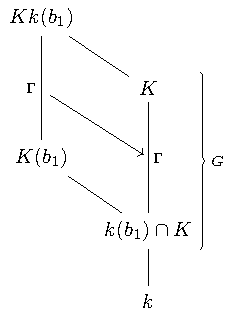
\includegraphics{commu/commu3.pdf}
				
			\end{minipage}
			\label{pic:galois}
		\end{figure}
		
		
		\item 这个方程的根$[r_1:r_2:\cdots:r_5]$显然落在二次曲面
		$$\mathcal{Q}:=\left\{[r_1:r_2:\cdots:r_5] \in \mathbb{PC}^4 \,\middle|\, \sum_{i=1}^{5}r_i=\sum_{i=1}^{5}r_i^2=0 \right\}$$
		中.由于它是$\mathbb{PC}^3$中的满秩曲面,故同构于$\mathbb{PC}^1 \times \mathbb{PC}^1$.另外我们也有三次曲面
		$$\mathcal{C}:=\left\{[r_1:r_2:\cdots:r_5] \in \mathbb{PC}^4 \,\middle|\, \sum_{i=1}^{5}r_i=\sum_{i=1}^{5}r_i^3=0 \right\},$$
		这两个曲面在约化过程中将起到重大作用,尤其是曲面$\mathcal{Q}$.
	\end{itemize}
\end{remarks}

若通过更进一步的Jerrard-Bring约化,则可以通过解额外的辅助方程\footnote{参见\cite{green1978on},自然仍需添入额外的二次/三次根.}将方程\eqref{eq:firstreduction}化为
$$x^5-x+\gamma=0 \quad \text{or} \quad x^5+\gamma=0\;\text{(easy!)}$$
的形式,前一种被称为Bring-Jarrard form,此为一路.

另外一路,我们将按照\cite[5.8]{shurman1997geometry}的流程,将方程\eqref{eq:firstreduction}化为\eqref{eq:brioschi}的形式.设原方程为
$$p(T):=T^5-\sigma_3 T^2+\sigma_4 T -\sigma_5$$
通过定义满足一定限制的多项式$t(T) \in k[T] \; \big(\hspace{-0.25cm}\mod p(T)\big)$,我们得到新的五次方程
\begin{equation}\label{eq:closetoBri}
q(T):=\prod_{i=1}^{5} (T-t(r_i))=T^5+d_1T^4+d_2T^3+d_3T^2+d_4T+d_5 \in k[T]
\end{equation}
简化后得到Brioschi预解式.这个过程的难点在于复杂的代数构造:
\begin{enumerate}[Step 1.]
	\item 构造三次或四次首一多项式$\psi(T) \in k[T]$,使得\footnote{主要的思路是配凑,可参见\cite[exercise 5.8.1]{shurman1997geometry}}
	$$\sum \psi(r_i)=\sum \psi(r_i)^2=\sum r_i\psi(r_i)=0$$
	这样我们才能令$\mathbb{C}^2$以如下方式作用于曲面$\mathcal{Q}$:
	$$(a,b) \longmapsto [r_i \mapsto ar_i+b\psi(r_i)]$$
	\item 将域$k[T]/(p(T))$视作5维$k$-线性空间,则$T^2,\psi(T) T ,\psi(T)^2, T,\psi(T),1$线性相关,故有非零等式
	$$\alpha T^2+2\beta T \psi +\gamma \psi^2 -aT-b\psi+c=0 	\qquad \text{in $k[T]$}$$
	通过代入$T=r_i$后求和得到$c=0$,从而令
	\begin{equation*}
	\begin{aligned}
	L(X,Y):=&\,aX+bY=\begin{pmatrix}
	a&b
	\end{pmatrix}
	\begin{pmatrix}
	X\\Y
	\end{pmatrix}\\
	Q(X,Y):=&\,\alpha X^2+2\beta XY+\gamma Y^2=\begin{pmatrix}
	X & Y
	\end{pmatrix}
	\begin{pmatrix}
	\alpha & \beta\\
	\beta & \gamma
	\end{pmatrix}
	\begin{pmatrix}
	X \\ Y
	\end{pmatrix}
	\end{aligned}
	\end{equation*}
	我们得到
	\begin{itemize}
		\item $L(T,\psi(T))\equiv Q(T,\psi(T)) \quad \text{mod } p(T)$
		\item $L,Q$均不为$0$多项式,且$L(T,\psi(T))\equiv Q(T,\psi(T)) \neq 0 \quad \text{mod } p(T)$.
		\item $L \nmid Q \text{ in }k[X,Y]$ 
		\item $m:=Q(b,-a), \quad \delta:=\alpha\gamma-\beta^2$均不为零.
	\end{itemize}
	\item 先承认一个引理:
	\begin{lemma}\label{lem:matrixproof}
		设$L$, $Q$, $m$, $\delta$如上所示,且$L \nmid Q$.那么,存在单项式$\tilde{L}:=\tilde{a}X+\tilde{b}Y \in k[X,Y]$,使得
		\begin{equation}\label{eq:matrixproof}
		mQ(X,Y)=\tilde{L}(X,Y)^2+\delta L(X,Y)^2.
		\end{equation}
	\end{lemma}
	作为推论,我们有
	$$mL \equiv mQ =\tilde{L}^2 +\delta L^2=(\tilde{L}+\sqrt{-\delta}L)(\tilde{L}-\sqrt{-\delta}L) 	\qquad \text{in }k(\sqrt{-\delta})[T]$$
	在这之后我们终于可以给出多项式$t(T):=\tilde{L}(T,\psi(T)) \cdot L^{-1}(T,\psi(T))$(在模$p$意义下),且$t$满足
	\begin{equation*}
	\begin{aligned}
	t\equiv (1+\sqrt{-\delta}L_1)L_1^{-1} \; \text{ mod }p \qquad L_1:=(\tilde{L}+\sqrt{-\delta}L)/m\\
	t\equiv (1-\sqrt{-\delta}L_2)L_2^{-1} \; \text{ mod }p \qquad L_2:=(\tilde{L}-\sqrt{-\delta}L)/m\\
	\end{aligned}
	\end{equation*}
	\item 我们验证多项式\eqref{eq:closetoBri}即是我们所求的多项式.由于
	$$0=q\big(t(r_i)\big)=q\big(t(L_1(r_i))\big)=q(L_1)\big(r_i\big),$$
	展开得到
	$$L_1^5q(L_1)= \Big((1+\sqrt{-\delta}L_1)^5+d_1 L_1 (1+\sqrt{-\delta}L_1)^4 + \cdots + d_5 L_1^5\Big)$$
	中的$3$, $4$次系数均为$0$,由此得到多项式$q$系数的$2$个线性函数.对$q(L_2)$采用同样的操作,解完方程组后得到
	$$q=T^5+\frac{10}{3}\delta T^3+5\delta^2T+d_5$$
	最后令$\displaystyle S:=-\frac{\delta^2}{9d_5}T$, $\;\displaystyle W:=-\frac{\delta^5}{3^5 \cdot d_5^2}$,得到Brioschi预解式:
	$$q(S)=S^5-10WS^3+45W^2S-W^2$$
	\item \begin{proof}[引理\ref{lem:matrixproof}的证明]\
		假设我们已经找出$\tilde{L}$,将方程写成矩阵形式:
		\begin{equation*}
		\begin{aligned}
		mQ(X,Y)=&\tilde{L}(X,Y)^2+\delta L(X,Y)^2\\
		\Longleftrightarrow\; m\begin{pmatrix}
		\alpha & \beta \\ \beta & \gamma
		\end{pmatrix}=&
		\begin{pmatrix}
		\tilde{a} \\ \tilde{b}
		\end{pmatrix}
		\begin{pmatrix}
		\tilde{a} & \tilde{b}
		\end{pmatrix}
		+\delta
		\begin{pmatrix}
		a \\ b
		\end{pmatrix}
		\begin{pmatrix}
		a & b
		\end{pmatrix}\\
		=& 
		\begin{pmatrix}
		\tilde{a} & a \\ \tilde{b} & b
		\end{pmatrix}
		\begin{pmatrix}
		1 & 0 \\ 0 & \delta
		\end{pmatrix}
		\begin{pmatrix}
		\tilde{a} & \tilde{b} \\ a & b
		\end{pmatrix}
		\end{aligned}
		\end{equation*}
		取$\tilde{a}:=a\beta-b\alpha$, $\tilde{b}:=a\gamma-b\beta$即可满足条件.
	\end{proof}
\end{enumerate}


\section{通过模形式解五次方程}
若是只要求形式幂级数解,则对方程\eqref{eq:Bring-Jarrard}有一个组合得到的解:
$$x(\gamma) = \sum_{k=0}^{\infty} \binom{5k}{k} \frac{\gamma^{4k+1}}{4k+1}$$
那么我们的故事就结束了.不过,这样直接的解总是显得不太自然.或者说,这不过是为路人提供的人为捷径,而真正的探险者则有意避开,为的就是在那危峰兀立的山崖上,瞥见常人所不能识的自然之美.
%如果你愿意追随,那么,我们将会用正二十面体方程来解一般的五次方程(or 将一般的五次方程化为正二十面体方程),再用模形式来解正二十面体方程.这样看,正二十面体方程则是五次方程的一个``典型代表",而它的模形式解则不过是图\ref{fig:tran}中辅助方程的一个类比.

记$$\Gamma(N):=\left\{ \begin{pmatrix}
a &b \\ c & d
\end{pmatrix} \in SL_2(\mathbb{Z}) \;\middle|\; \begin{pmatrix}
a &b \\ c & d
\end{pmatrix} \equiv \begin{pmatrix}
1 &0 \\ 0 & 1
\end{pmatrix} \mod N  \right\}$$
特别地, $\Gamma(1)=SL_2(\mathbb{Z})$,我们有正合列

\begin{center}
	\begin{tikzcd}
		1 \arrow[r]           & \Gamma(5) \arrow[r]             & PSL_2(\mathbb{Z}) \arrow[r]   & PSL_2(\mathbb{F}_5) \arrow[d, "\sim"] \arrow[r] & 1 \\
		&                  &     & {\Gamma_{(2,3,5)}}                              &   \\
		\mathcal{H} \arrow[r] & \mathcal{H}/\Gamma(5) \arrow[r] & \mathcal{H}/\Gamma(1) &                                                 &  
	\end{tikzcd}
\end{center}
\vspace{-2cm}\text{从而得到}\\[1.5cm]
诱导的交换图($\mathcal{H}^*:=\mathcal{H} \cup \mathbb{Q}^*$)

\begin{center}
	\begin{tikzcd}
		\mathcal{H}^* \arrow[r, "r"] & \mathcal{H}^*/\Gamma(5) \arrow[r, "\pi_1"] \arrow[d, "\hat{j}_5","\sim"'] & \mathcal{H}^*/\Gamma(1) \arrow[d, "\hat{j}","\sim"'] \\
		& \mathbb{PC}^1 \arrow[r, "I"]                                      & \mathbb{PC}^1                               
	\end{tikzcd}
\end{center}
我们留给下一章的任务:
\begin{enumerate}
	\item 构造$j_5:\mathcal{H}^* \longrightarrow \mathbb{PC}^1 $,证明其诱导的$\hat{j}_5:\mathcal{H}^*/\Gamma(5) \longrightarrow \mathbb{PC}^1$为同构;
	\item 构造$I:= \hat{j} \circ \pi_1 \circ \hat{j}_5^{-1}$,验证其满足$I=1728Z_5$,从而得到
	$$Z_5^{-1}=\frac{1}{1728}I^{-1}=\frac{1}{1728}j_5 \circ j^{-1}$$
	从而通过模方程$j(\tau)=j_0$的解得到正二十面体方程的解.
\end{enumerate}
  
\chapter{模形式与模曲线}
\section{经典模形式回顾}
我们从与模形式密切相关的复环面开始谈起.
\subsection{复环面}

给定$\tau \in \mathcal{H}$,取格点$\Lambda_{\tau}:= \mathbb{Z}\tau \oplus \mathbb{Z} \!\cdot\!\! 1$,则复环面自然成为紧黎曼面,亏格为1.定义\textbf{Weierstrass函数}\footnote{$\sum'$表示对0以外的点求和.}
$$\wp_{\Lambda_{\tau}}(z):=\frac{1}{z^2}+ \summ_{w \in \Lambda_{\tau}}\left( \frac{1}{(z-w)^2}-\frac{1}{w^2} \right)$$
则上述级数在$\mathbb{C} \smallsetminus \Lambda_{\tau}$的紧子集中一致收敛,故$\wp_{\Lambda_{\tau}}(z)$为$\mathbb{C}$上良定的亚纯函数. $\wp_{\Lambda_{\tau}}(z)$有周期$1$, $\tau$, 故$\wp_{\Lambda_{\tau}}$可视作复环面上的亚纯函数.可以证明$\mathbb{C}/\Lambda_{\tau}$上的亚纯函数空间为
$$\mathcal{M}(\mathbb{C}/\Lambda_{\tau})=\mathbb{C}(\wp,\wp') \cong \mathbb{C}(x)[y]/(-y^2+4x^3-g_2x-g_3)\quad g_2,g_3 \in \mathbb{C}. $$

复环面可以通过射影嵌入
$$\mathbb{C}/\Lambda_{\tau} \longrightarrow \mathbb{PC}^2 \qquad \bar{z} \longmapsto \begin{cases}
[\wp,\wp',1], & z \notin \Lambda_{\tau} \\
[0,1,0], & z \in \Lambda_{\tau}
\end{cases} $$
成为$\mathbb{PC}^2$中的射影簇,称为复椭圆曲线.由下图示过程可以得到复环面,亏格为1的紧黎曼面和复椭圆曲线的等价性,详尽解释可参考\cite[第八章]{Li2019modularform}.
\begin{figure}[ht]
	\centering
		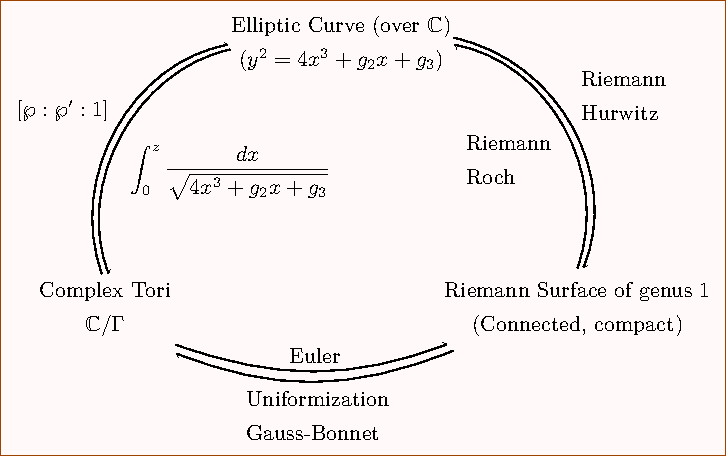
\includegraphics[width=0.8\textwidth]{Flowchart/Ellipticcurve.pdf}
	\label{pic:Ellipticcurve}
\end{figure}

\subsection{模空间$\mathcal{H}/SL_2(\mathbb{Z})$}
现在我们扰动点$\tau \in \mathcal{H}$,得到不同的复环面.在黎曼面范畴同构的意义下,
$$\Lambda_{\tau} \cong \Lambda_{\tau'} \Longleftrightarrow \text{存在$\gamma \in SL_2(\mathbb{Z})$,使得$\gamma \tau = \tau'$}$$
故所有复环面构成的空间为$\mathcal{H}/SL_2(\mathbb{Z})$,在加入尖点紧化后同构于$\mathbb{PC}^1$.为了定义``模空间中的函数(截面)",我们引进模形式的概念:

\begin{defn}
	称$\mathcal{H}$上的全纯函数$f$为权$k \in \mathbb{Z}$,级$\Gamma:= SL_2(\mathbb{Z})$的模形式,若
	
	\begin{enumerate}[(1)]
		\item 对任意$\gamma=\begin{pmatrix}
		a & b\\
		c & d
		\end{pmatrix}\in \Gamma$,均有
		\begin{equation}\label{eq:modform}
		f(\gamma \tau)=(c \tau +d)^k f(\tau)
		\end{equation}
		特别地,我们有$f(\tau+1)=f(\tau)$.
		\item $f$的Fourier展开$f(\tau)=\sum_{n \in \mathbb{Z}}a_ne^{2\pi i n \tau}$中,对$n < 0$, $a_n =0$.\footnote{一个直观的看法:取$\infty$附近的局部坐标为$q:=\exp(2\pi i \tau)$,则该条件等价于$f$在$\infty$全纯.}
	\end{enumerate}
	记权为$k$,级为$\Gamma$的模形式构成的空间为$\operatorname{M}_k(\Gamma)$, $\operatorname{M}_{*}(\Gamma):= \oplus_{k \in \mathbb{Z}}\operatorname{M}_k(\Gamma)$为对应的分次环.
	
	若额外要求$(2)$中的$a_0=0$ ($\infty$为截影$f$的零点),则称其为尖点形式,及其构成的空间为$\operatorname{S}_k(\Gamma)$, $\operatorname{S}_{*}(\Gamma):= \oplus_{k \in \mathbb{Z}}\operatorname{S}_k(\Gamma)$为对应的分次环.
\end{defn}

\begin{exercise}
	对于$k \in \mathbb{Z}$, $k>2$,定义\textbf{Eisenstein函数}
	$$G_k(\tau):= \frac{1}{2}\summ_{w \in \Lambda_{\tau}} \frac{1}{w^k}=\frac{1}{2} \summ_{(m,n) \in \mathbb{Z}^2} \frac{1}{(m\tau +n)^k}$$
	其中$\sum'$表示对0以外的点求和,可以验证
	\begin{enumerate}
		\item 级数在$\mathcal{H}$的紧子集上一致收敛, $G_k$为$\mathcal{H}$上的全纯函数;
		\item $k$为奇数时, $G_k \equiv 0$;
		\item $k$为偶数时, $G_k$满足\eqref{eq:modform},且有Fourier展开
		$$G_k(\tau)=\frac{(2\pi i)^k}{(k-1)!} \left( -\frac{B_k}{2k}+\sum_{n=1}^{\infty}\sigma_{k-1}(n)q^n \right)$$
		故$G_k$为权$k$,级$SL_2(\mathbb{Z})$的模形式.
	\end{enumerate}
\end{exercise}

为方便起见,取$E_k:= G_k/(2\zeta(k))$使得Fourier常数项化为1.可以证明, $M_{*}(SL_2(\mathbb{Z}) \cong \mathbb{C}[E_4,E_6])$,且$E_4,E_6$代数无关.

\begin{remark}
	模形式可视作格点上的函数,即
	$$F: \{\Lambda= \mathbb{Z}e_1 \oplus \mathbb{Z}e_2 \} \longrightarrow \mathbb{C} \qquad \Lambda \longmapsto F(\Lambda)$$
	满足$F(\lambda \Lambda)= \lambda^{-k} F(\Lambda)$
	
	取$f(\tau):=F(\Lambda_{\tau})$,则有
	\begin{equation*}
	\begin{aligned}
	f(\gamma \tau) =\, & F(\Lambda_{\gamma\tau})=F(\mathbb{Z}\gamma\tau \oplus \mathbb{Z} \!\cdot\!\! 1)\\
	=\,& (c\tau + d)^k F\big(\mathbb{Z}(a\tau+b) \oplus \mathbb{Z}(c\tau +d)\big)		\\
	=\,& (c\tau + d)^k F(\Lambda_{\tau})		\\
	=\,& (c\tau + d)^k f(\tau)		\\
	\end{aligned}
	\end{equation*}
	事实上,我们也是通过上述方式来构造Eisenstein级数的.
\end{remark}
\begin{figure}[ht]
		\centering
		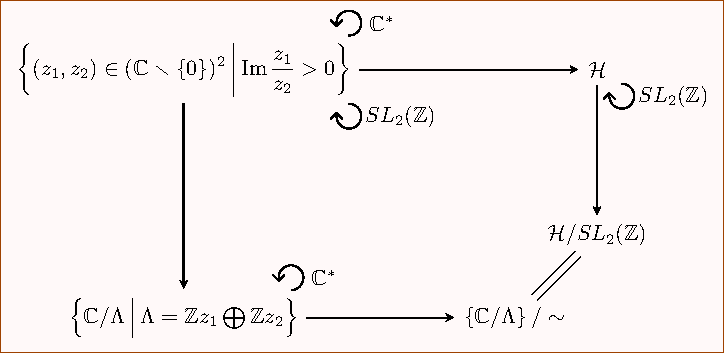
\includegraphics[width=0.8\textwidth]{Flowchart/Modularcurve.pdf}
	\caption{构造模空间/模形式的过程}
	\label{pic:Modularcurve}
\end{figure}
另外补充两个重要的函数:模判别式
$\Delta:=\frac{1}{1728}(E_4^3-E_6^2)$
给出了第一个在$\infty$处取0的模形式,由它可以得到尖点形式的结构;$j:=E_4^3/\Delta$给出紧化的模空间$\mathcal{H}^*/SL_2(\mathbb{Z})$至$\mathbb{PC}^1$的黎曼面同构.\footnote{注意$j$不是模形式,它在$\infty$处有1阶极点.}

我们以一个表\ref{tb:torus-moduli}作为上述内容的总结:
\begin{table}[ht]
	\centering
	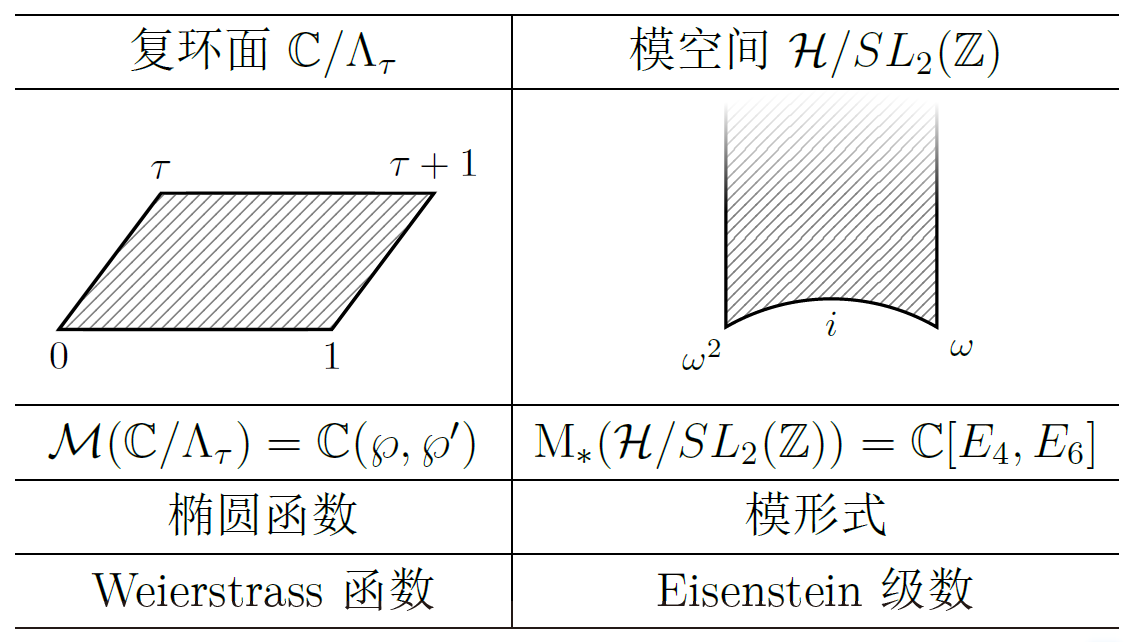
\includegraphics[width=0.6\textwidth]{snip/table-torus-moduli.png}
	\caption{复环面与模空间的比较}
	\label{tb:torus-moduli}
\end{table}
\subsection{Jacobi模形式}
曾经我突发奇想,是否存在一个$\mathcal{H}/SL_2(\mathbb{Z})$上的纤维丛$E$,使得每一个点$\tau$对应的纤维$E_\tau$恰好就是复环面$\mathbb{C}/\Lambda_{\tau}$?直到有一天我找到了梦中的空间:
$$E:=SL_2(\mathbb{Z})\textbackslash (\mathcal{H} \times \mathbb{C})/\mathbb{Z}^2 \qquad \gamma(\tau,z):= (\gamma \tau,\frac{z}{c\tau +d}) \quad (m,n)(\tau,z):=(\tau, z+m\tau+n)$$
这个空间鼓励我们通过整体的方式来看问题,让我们回顾Weierstrass函数$\wp(z,\tau):= \wp_{\Lambda_{\tau}}(z)$,发现它可以视作两个变元的函数,并且它的Laurent展开
$$\wp(z,\tau)=\frac{1}{z^2}+ \sum_{k=1}^{\infty}(2k+1) G_{2(k+1)}(\tau)z^2$$
中的系数即是经典的模形式.或许作为Weierstrass函数也可以称作某种特殊的模形式?在下一节我们将给出Weierstrass函数的一系列``同类"——$\theta$-函数,它们被统称为Jacobi模形式.
%\begin{defn}
%	我们称亚纯函数$f:\mathbb{C} \times \mathcal{H} \longrightarrow \mathbb{C}$为Jacobi模形式,若
%	\begin{enumerate}[1.]
%		$f$
%	\end{enumerate}
%\end{defn}

%引入向量丛,
%老话常谈的材料中要加入Weierestrass函数的展开是Jacobi模形式,这也是某个$\theta$函数,意味着我们开始讨论“所有复环面”
%Jacobi模形式的定义

\subsection{级结构}
下一步,我们要推广模形式的定义,考虑复环面的级结构,将级从$SL_2(\mathbb{Z})$推广到同余子群
$$\Gamma(N):=\left\{ \begin{pmatrix}
a &b \\ c & d
\end{pmatrix} \in SL_2(\mathbb{Z}) \;\middle|\; \begin{pmatrix}
a &b \\ c & d
\end{pmatrix} \equiv \begin{pmatrix}
1 &0 \\ 0 & 1
\end{pmatrix} \mod N  \right\}$$
上. (还记得上章末尾留的任务吗?)简要一提,这个群有一个经典的正合列: ($N>3$)
\begin{center}
	\begin{tikzcd}
		1 \arrow[r]           & \Gamma(N) \arrow[r]             & PSL_2(\mathbb{Z}) \arrow[r]   & PSL_2(\mathbb{Z}/N\mathbb{Z}) \arrow[r] & 1 
	\end{tikzcd}
\end{center}

我们定义$\mathcal{H}/\Gamma(N)$的尖点为$\mathbb{PQ}^1 /\Gamma(N)$,有一些不太显然的性质\footnote{参考\cite[练习1.4.14,2.5,例4.2.2]{Li2019modularform}}:
\begin{itemize}
	\item 我们有群的阶数
	$$\mu(N):= \# \,PSL_2(N) =\begin{cases}\displaystyle
	\frac{N^3}{2} \prod_{p \mid N}(1-p^{-2}), & N>2\\
	6, & N=2
	\end{cases}$$
	\item $N>1$时, $\Gamma(N)$无椭圆点,复叠映射$\mathcal{H} \longrightarrow\mathcal{H}/\Gamma(N)$为非分歧映射; $\mathcal{H}/\Gamma(N)$在标准双曲度量下面积为
	$\frac{\pi}{3} \mu$.
	\item $\Gamma(1)=SL_2(\mathbb{Z})$在$\mathbb{PQ}^1$上的作用可递,故$\mathcal{H}/\Gamma(1)$的尖点为独点集,记为$\infty$.
	\item 模空间$\mathcal{H}/\Gamma(N)$加入所有尖点后成为紧黎曼面,亏格为
	$$g(N)=\begin{cases}\displaystyle
	1+ \frac{N^2(N-6)}{24} \prod_{p \mid N}(1-p^{-2}), & N >2\\
	0, & N=2
	\end{cases}$$
	其在$\infty$附近的局部坐标为$q:=\exp(2\pi i \tau/N)$;其他尖点通过$\Gamma(1)$的可递作用表示为$\gamma^{-1} \infty$,附近的局部坐标为$\exp(2\pi i \gamma(\tau)/N)$.
	\item 我们有尖点清晰的代数刻画:记
	$$(\mathbb{Z}/N\mathbb{Z})^2_{\prim}:=\left\{(a,b) \in (\mathbb{Z}/N\mathbb{Z})^2 \middle| (a,b)\text{ 为$N$阶元} \right\}$$
	则有$\Gamma(1)$-等变同构\footnote{需要注意这里对取的代表元有限制,要求$x$, $y$互质.}:( $\phi\big((x,y)\gamma\big)=\gamma^{-1}\phi\big((x,y) \big)$ )
	\begin{equation}\label{eq:cusppointiso}
	\phi\colon\pm\textbackslash(\mathbb{Z}/N\mathbb{Z})^2_{\prim} \longrightarrow \{ \Gamma(N) \text{ 的尖点}\} \qquad \overline{(x,y)} \longmapsto \overline{-y/x}
	\end{equation}
	通过这个同构,可以直接算出所有尖点的位置以及尖点的元素个数
	$$n(N)=\begin{cases}\displaystyle \;
	\frac{N^2}{2}  \prod_{p \mid N} (1-p^{-2}), & N >2\\
	\;\;3, & N=2
	\end{cases}$$
\end{itemize}
	在之后,我们记$Y(\Gamma(N)):= \mathcal{H}/\Gamma(N)$, $X(\Gamma(N))$为$Y(\Gamma(N))$紧化后得到的复黎曼面.
\begin{remark}
	类似于$\mathcal{H}/SL_2(\mathbb{Z})$,可以证明$Y(\Gamma(N))$分类了对象
	$$(\Lambda, \alpha: (\mathbb{Z}/N\mathbb{Z})^2\overset{\sim}{\longrightarrow} E_{\Lambda}[N] )/\sim$$
	其中$E_{\Lambda}[N]:=\left\{ z \in \mathbb{C}/\Lambda \middle| Nz=0 \right\}$.
\end{remark}



\begin{defn}
	称$\mathcal{H}$上的全纯函数$f$为权$k \in \mathbb{Z}$,级$\Gamma:= \Gamma(N)$的模形式,若
	
	\begin{enumerate}[(1)]
		\item 对任意$\gamma=\begin{pmatrix}
		a & b\\
		c & d
		\end{pmatrix}\in \Gamma$,均有
		\begin{equation}\label{eq:modform2}
		f(\gamma \tau)=(c \tau +d)^k f(\tau)
		\end{equation}
		特别地,我们有$f(\tau+N)=f(\tau)$.
		\item $f$在所有尖点处全纯.
	\end{enumerate}
	记权为$k$,级为$\Gamma$的模形式构成的空间为$\operatorname{M}_k(\Gamma)$, $\operatorname{M}_{*}(\Gamma):= \oplus_{k \in \mathbb{Z}}\operatorname{M}_k(\Gamma)$为对应的分次环.
	
	若额外要求函数$h$在所有尖点处消没,则称其为尖点形式,及其构成的空间为$\operatorname{S}_k(\Gamma)$, $\operatorname{S}_{*}(\Gamma):= \oplus_{k \in \mathbb{Z}}\operatorname{S}_k(\Gamma)$为对应的分次环.
\end{defn}
\begin{remark}
	事实上我们需要的定义比这广泛得多:我们将考虑带特征的半整权模形式,并将尖点处要求放松为``极点"\footnote{我们之后只会考虑这个空间具体的函数和特殊的子空间,其在尖点处的性质均可以计算,故定义的空间再大一些也无所谓.}.读者可以将其同第\ref{sec:inva}节中的$\Gamma'$-半不变量作类比.
\end{remark}
\begin{defn}
	称$\mathcal{H}$上的全纯函数$f$为权$k \in \frac{1}{2}\mathbb{Z}$,级$\Gamma:= \Gamma(N)$,特征$\bigchi$的模形式,若对任意$\gamma=\begin{pmatrix}
	a & b\\
	c & d
	\end{pmatrix}\in \Gamma$,均有
	\begin{equation}\label{eq:modform3}
	f(\gamma \tau)=\bigchi(\gamma)(c \tau +d)^k f(\tau)
	\end{equation}
\end{defn}
\begin{remark}
	当$k \in \frac{1}{2} \mathbb{Z} \smallsetminus \mathbb{Z}$时, $(c\tau+d)^k$开根的问题可以被``吸附"至特征$\bigchi$中,故我们只需取一个一致的单值解析分支使得$1^{1/2}=1$即可.
\end{remark}
%然后重点是提出主同余子群,略述其定义、模空间紧化、尖点的内容,



%直接承认无椭圆点,,指数,亏格公式和尖点个数,列表.

\section{$\theta$-函数}
\subsection{定义}
作为研究经典模形式的有力武器,同时也作为Jacobi模形式的极典型例子,我们引入$\theta$-函数的定义:

\begin{defn}
	我们定义带特征$\chi:=\normalcharacter \in \mathbb{R}^2$的$\theta$-函数
	$$\theta\normalcharacter : 
	\mathbb{C} \times \mathcal{H} \longrightarrow \mathbb{C}$$
	$$\theta\normalcharacter(z, \tau)=\sum_{n \in \mathbb{Z}} \exp 2 \pi i \left\{\frac{1}{2}\left(n+\frac{\epsilon}{2}\right)^{2} \tau+\left(n+\frac{\epsilon}{2}\right)\left(z+\frac{\epsilon^{\prime}}{2}\right)\right\}$$
	
	注意到$\theta$-函数的良定性,且分别关于$z$, $\tau$全纯.
\end{defn}
\subsection{恒等式}
我们在此处不加证明地引用$\theta$-函数的一部分恒等式,这些恒等式的导出均初等,却需要足够的代数成熟度.在这里我们强烈建议对证明感兴趣的读者按着\cite[Chapter2.1]{farkas2001theta}中的步骤一步步推导.
\subsubsection{基本公式}
\begin{gather*}
\intertext{关于$\chi$:}
\theta\normalcharacter(z, \tau)=\exp 2 \pi  i \left\{\frac{1}{8} \epsilon^{2} \tau+\frac{1}{2} \epsilon z+\frac{1}{4} \epsilon \epsilon^{\prime}\right\} \theta\character{0}{0}\left(z+\frac{\epsilon^{\prime}}{2}+\frac{\epsilon}{2} \tau, \tau\right) \tag*{[2.3]} \label{eq:chieq}\\
\theta \character{\epsilon+2m}{\epsilon'+2n}(z,\tau)=\exp(\pi i \epsilon n)\, \theta \normalcharacter (z,\tau)\tag*{[2.9]} \\
	\theta \character{-\epsilon}{-\epsilon'}(z,\tau)= \theta \normalcharacter(-z,\tau)	
\tag*{[2.10]}
\end{gather*}
\begin{gather*}
\intertext{关于$(z)$的平移:\footnotemark}
\theta\normalcharacter(z+n+m \tau, \tau)=\exp 2 \pi  i \left\{\frac{n \epsilon-m \epsilon^{\prime}}{2}-m z-\frac{m^{2}}{2} \tau\right\} \theta\normalcharacter(z, \tau) \tag*{[2.4]}\label{eq:Translation}
\end{gather*}
\footnotetext{$n,m \in \mathbb{Z}$.}
\begin{gather*}
\intertext{关于$(\tau)$的变换公式:\footnotemark}
%\frac{\exp \pi  i \left\{\frac{-c z^{2}}{c \tau+d}\right\} \theta\normalcharacter\left(\frac{z}{c \tau+d}, \frac{a \tau+b}{c \tau+d}\right)}{\theta \character{a \epsilon+c \epsilon^{\prime}-a c}{b \epsilon+d \epsilon^{\prime}+b d}(z, \tau)}=\kappa\left(\normalcharacter, \gamma\right)(c \tau+d)^{\frac{1}{2}}
\hspace{-3cm}\theta\normalcharacter\left(\frac{z}{c \tau+d}, \frac{a \tau+b}{c \tau+d}\right) =\kappa\left(\normalcharacter, \gamma\right)(c \tau+d)^{\frac{1}{2}} \\
\hspace{3cm}\times \exp \pi  i \left\{\frac{c z^{2}}{c \tau+d}\right\} \theta \character{a \epsilon+c \epsilon^{\prime}-a c}{b \epsilon+d \epsilon^{\prime}+b d}(z, \tau)
\tag*{[2.16]}\label{eq:Transformation}
\intertext{其中$\kappa\left(\character{0}{0}, \gamma \right)$为八次单位根,只依赖于$\gamma$;而}
\hspace{-8cm}\kappa\left(\normalcharacter, \gamma\right)= \kappa\left(\character{0}{0}, \gamma\right) \\
\hspace{3cm}\times\exp 2 \pi  i \left\{-\frac{1}{4}\left(a \epsilon+c \epsilon^{\prime}\right) b d-\frac{1}{8}\left(a b \epsilon^{2}+c d \epsilon^{\prime 2}+2 b c \epsilon \epsilon^{\prime}\right)\right\}  \tag*{[2.17]}\label{eq:Transformation2}
\end{gather*}

\footnotetext{$\gamma=\left(\begin{smallmatrix}
	a & b\\ c & d
	\end{smallmatrix}\right) \in SL_2(\mathbb{Z})$}
\subsubsection{方程相关公式}
\begin{gather*}
\intertext{函数方程:($\theta$-函数的另一种定义)固定$\tau$, $\chi$,令$f(z):=\theta \normalcharacter(z,\tau)$,则}
f(z+1, \tau)=\exp (\pi  i  \epsilon) f(z, \tau) 	\tag*{[2.5]}\\
f(z+\tau, \tau)=\exp \left(-\pi  i \left\{\epsilon^{\prime}+2 z+\tau\right\}\right) f(z, \tau)	\tag*{[2.6]}	
\intertext{热方程(物理意义):简记$':=\partial_z$,则}
\theta'' \normalcharacter (z,\tau) =4\pi i \frac{\partial \theta}{\partial \tau} \normalcharacter (z,\tau)	\tag*{[p73]}
\intertext{Fourier展开:记$w:=\exp (2\pi iz)$,则}	
\theta \normalcharacter (z,\tau) =\omega^{\textstyle\frac{\epsilon}{2}} \sum_{n\in \mathbb{Z}}a_n\omega^n	\tag*{[2.7]}
\intertext{其中}
a_{n}=\exp 2\pi i \left\{ \frac{1}{2} \left(n+\frac{\epsilon}{2}\right)^2 \tau + \left(n+\frac{\epsilon}{2}\right) \frac{\epsilon'}{2}  \right\}
\end{gather*}

\subsubsection{乘积公式}
记$w:=\exp (2\pi iz)$, $q=\exp (2\pi i \tau)  $,则\footnote{在许多书中均取$q=\exp \{\pi i \tau \}$,但我们统一取$q=\exp \{2 \pi i \tau\}$,希望读者不要混淆.}
\begin{equation*}
	\begin{aligned}
	\theta \character{0}{0}(z,\tau)=\;& \sum_{n \in \mathbb{Z}}q^{\frac{n^2}{2}}w^n\\
	=\;& \prod_{n=1}^{\infty}(1-q^n)\left( 1+q^{\frac{2n-1}{2}}w \right) \left( 1+\frac{q^{\frac{2n-1}{2}}}{w} \right)
	\end{aligned}
\end{equation*}
作为推论,我们有
$$\sum_{n \in \mathbb{Z}} (-1)^n x^{\frac{kn^2+ln}{2}}=\prod_{n=0}^{\infty} \left(1-x^{kn+\frac{k-l}{2}} \right)\left(1-x^{kn+\frac{k+l}{2}} \right)\left(1-x^{kn+k} \right)$$
并且由\ref{eq:chieq},所有的$\theta$-函数均有对应的乘积公式。
\subsubsection{散在恒等式}
%在书中还有一些散在恒等式,也在此一并列下:
\begin{gather*}
\theta\normalcharacter(z, \tau)=\sum_{l=0}^{N-1} \theta\character{\frac{\epsilon+2 l}{N}}{N \epsilon^{\prime}}\left(N z, N^{2} \tau\right)	\tag*{[p76]} \\
\theta\normalcharacter(0, \tau) \theta\character{\delta}{ \delta^{\prime}} (0, \tau)   =\theta\character{\frac{\epsilon+\delta}{2}} {\epsilon^{\prime}+\delta^{\prime}} (0,2 \tau) \theta\character{\frac{\epsilon-\delta}{2}}   {\epsilon^{\prime}-\delta^{\prime}} (0,2 \tau)\\
\hspace{6.5cm}   +\theta\character{\frac{\epsilon+\delta}{2}+1}   {\epsilon^{\prime}+\delta^{\prime}} (0,2 \tau) \theta\character{\frac{\epsilon-\delta}{2}+1}   {\epsilon^{\prime}-\delta^{\prime}} (0,2 \tau)	\tag*{[2.15]} \\
\theta \normalcharacter (-z,\tau) =\exp (\pi i \epsilon \epsilon') \theta \normalcharacter (z,\tau) \qquad \text{当$\normalcharacter \in \mathbb{Z}^2$}	\tag*{[p76]} 
\end{gather*}
\begin{remarks}\
	\begin{enumerate}[1.]
		\item 含参是为了有更多的操作空间,取不同的特殊值则能得到更多更简洁优美的恒等式.例如,令$z=0$,我们得到\textbf{$\theta$-级数}\footnote{我们使用相同的符号,注意不要混淆.}:
		$$\theta \normalcharacter (\tau):=\theta \normalcharacter (0,\tau)$$
		特别地, $\theta \character{0}{0}$, $\theta \character{1}{0}$, $\theta \character{0}{1}$, $\theta \character{1}{1} \equiv 0$是人们所熟知的\textbf{Jacobi $\theta$-级数},例如:
		$$\theta \character{0}{0} (\tau) = \sum_{n \in \mathbb{Z}} q^{\textstyle \frac{n^2}{2}}=1+2q^{\textstyle \frac{1}{2}}+2q^{2} + 2q^{\textstyle \frac{9}{2}}+ \cdots$$
		我们简记其为$\theta_{00}(\tau)$, $\theta_{10}(\tau)$, $\theta_{01}(\tau)$, $\theta_{11}(\tau)$,它们之间有关系
		$$\theta_{00}^4=\theta_{01}^4+\theta_{10}^4$$
		
		有时我们也会用到含参数的Jacobi $\theta$-函数$\theta_{00}(z,\tau)$, $\theta_{10}(z,\tau)$, $\theta_{01}(z,\tau)$, $\theta_{11}(z,\tau)$,注意到他们都是关于$z$的奇/偶函数,这一点有助于在之后极大地简化计算过程(Taylor展开有一半为0).
		\item $\theta$函数除了拥有丰富的恒等式外,作为$z$的函数(固定$\chi, \tau$), $\theta \normalcharacter (z,\tau)$仅在$\displaystyle\frac{1-\epsilon'}{2}+\frac{1-\epsilon}{2}\tau + \Lambda_{\tau}$处有一阶零点.它同样可视作$\mathbb{C}/\Lambda_{\tau}$上某个向量丛的截影.这使得我们可以通过$\theta$函数来构造众多的模形式.
		\begin{table}[ht]
			\centering
			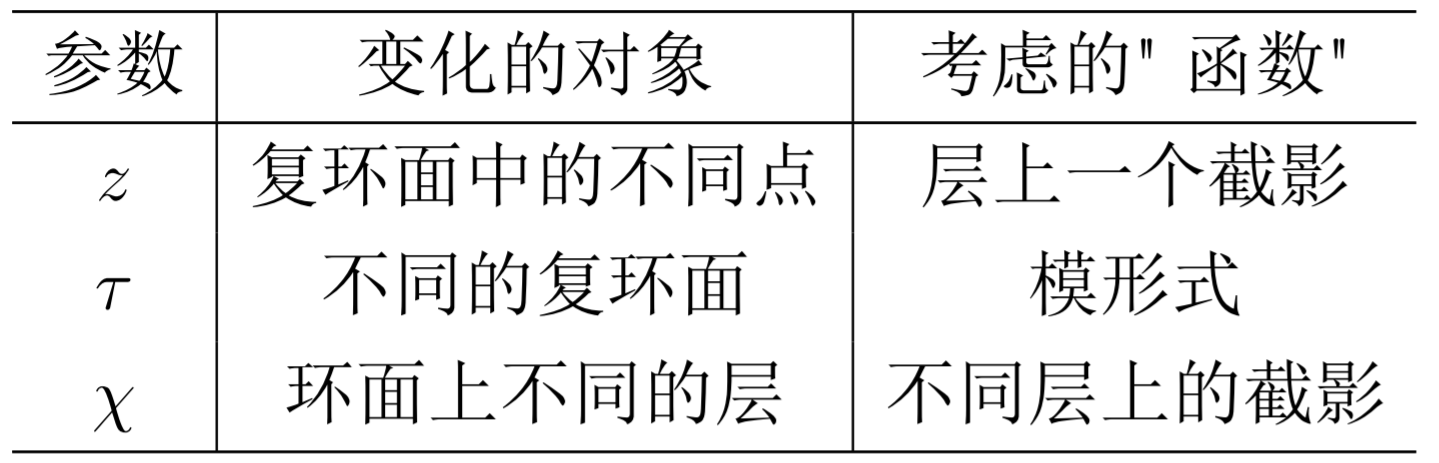
\includegraphics[width=0.5\textwidth]{snip/table-geomean.png}
			\caption{参数所代表的几何意义}
		\end{table}
		\item 恒等式不只是恒等式,它们有丰富的几何/算术性质.通过这种观点,我们将通过这些恒等式给出$X(\Gamma(N))$的性质.
	\end{enumerate}
	
\end{remarks}
%第二节引用,提出$\theta$函数,直接抄材料里的恒等式
\subsection{应用:表达$\wp$, $G_4$和$G_6$}
%小试牛刀,我们试着用$\theta$-函数来表达$\wp$, $G_4$和$G_6$.

\begin{theorem}[{\cite[Chapter 2, Theorem 5.10]{farkas2001theta}}]
	我们有表达
	\begin{equation}\label{eq:wpwiththeta}
	\wp_{\Lambda_{\tau}}(z) = - \left(\frac{\thetaaa{'}{z,\tau}}{\thetaaa{}{z,\tau}}\right)' +\frac{1}{3} \frac{\thetaaa{(3)}{0,\tau}}{\thetaaa{'}{0,\tau}}
	\end{equation}
\end{theorem}
\begin{proof}
	右式只在$\Lambda_{\tau}$处有二阶极点,比较两边在$0$处的Laurent展开即得.
\end{proof}
\begin{corollary}
	比较\eqref{eq:wpwiththeta}式两边系数得
	\begin{equation*}
	\begin{aligned}
	E_4(\tau)=\;&\frac{1}{18} \left(\frac{\thetaaatau{(3)}}{\thetaaatau{'}} \right)^2-\frac{1}{30} \frac{\thetaaatau{(5)}}{\thetaaatau{'}}\\
	E_6(\tau)=\;& \frac{1}{120} \frac{\thetaaatau{(3)}\thetaaatau{(5)}}{\thetaaatau{'}^2}-\frac{1}{108} \left(\frac{\thetaaatau{(3)}}{\thetaaatau{'}} \right)^3-\frac{1}{840} \frac{\thetaaatau{(7)}}{\thetaaatau{'}}
	\end{aligned}
	\end{equation*}
	$\Delta$, $j$亦可用$\theta$-级数表达.
\end{corollary}
\begin{exercise}
	固定$\tau \in \mathcal{H}$,试验证
	$$\mathbb{C}/\Lambda_{\tau} \longrightarrow \mathbb{PC}^2 \qquad z \longmapsto \left[\theta_{00}^2\theta_{11},\theta_{00}\theta_{01}\theta_{10},\theta_{11}^3 \right]$$
	为射影嵌入,得到$\mathbb{PC}^2$中的代数方程
	$$\theta_{00}^4 Y^2Z=X(\theta_{10}^2X-\theta_{01}^2Z)(\theta_{01}^2X+\theta_{10}^2Z).$$
\end{exercise}

%???然后把4个特殊的$\theta$函数列出来,说明其特殊性质(奇偶性(Taylor展开),四次恒等式,Jacobi导数公式,用$\theta$函数表示Weierestrass函数以及模形式,重新描述射影嵌入)
%还有$\eta$函数和乘积公式也可以顺手一提
%
%???Jacobi三/五乘积公式


\section{构造模形式}\label{sec:consofmodularform}

当我们想要进一步探讨如何用$\theta$-级数表达主同余子群的模形式时,一定会重新将焦点转移至公式\ref{eq:Translation}上.记$\chi:=\normalcharacter$, $\chi\gamma:=\character{a\epsilon+c\epsilon'-ac}{b\epsilon+d\epsilon'+bd}$,我们用更简练的语言来重新表达公式\ref{eq:Transformation}:
$$\exp \pi i \left\{ -cz^2\gamma'(\tau)^{\frac{1}{2}} \right\}\theta[\chi](z\gamma'(z)^{\frac{1}{2}},\gamma(\tau))=\kappa(\chi,\gamma)\gamma'(\tau)^{-\frac{1}{4}} \theta[\chi\gamma] (z,\tau)$$
取$z=0$,则有
\begin{equation}\label{eq:Transformation3}
\theta[\chi](0,\gamma(\tau))=\kappa(\chi,\gamma)\gamma'(\tau)^{-\frac{1}{4}} \theta[\chi\gamma] (0,\tau)
\end{equation}
当$\chi \gamma=\chi$时, $\theta[\chi](0,-)$成为权$1/2$,特征为$\kappa(\chi,-)$的模形式,然而这是在做梦.退而求其次,当$\chi\gamma \equiv \pm \chi \;(\!\!\!\!\mod (2\mathbb{Z})^2)$时,我们可以通过\ref{eq:Transformation2}调整公式\ref{eq:Translation},得到$\theta[\chi](0,\gamma(\tau))$同$\theta[\chi](0,\tau)$的关系.
\subsection{等价特征类空间}
\begin{defn}
	我们称特征类$\chi$与$\chi'$等价,若$\chi \equiv \pm \chi' \;(\!\!\!\!\mod (2\mathbb{Z})^2)$,记等价特征类的空间为$\mathds{X}:=\mathbb{R}^2/\sim$.
\end{defn}
\begin{figure}[ht]
	
	\begin{minipage}[t]{.9\textwidth}
		\vspace{0.1cm}
		\centering
		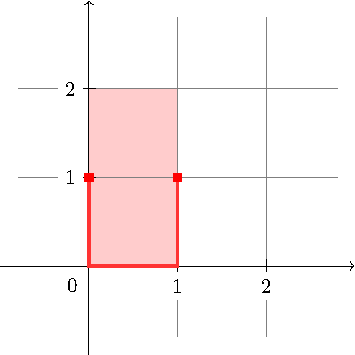
\includegraphics{pic/funsetofchar.pdf}
		
	\end{minipage}
	\caption{$\mathds{X}$所对应的基本集}
	\label{pic:basicsetofchar}
\end{figure}
\begin{defn}
	定义$\Gamma(1)$在$\mathds{X}$上的右作用
	$$\mathds{X} \times \Gamma(1) \longrightarrow \mathds{X} \qquad \normalcharacter \gamma := \character{a\epsilon+c\epsilon'-ac}{b\epsilon+d\epsilon'+bd}$$
	由于
	\begin{equation*}
	\begin{aligned}
	\normalcharacter \gamma =& \character{a(\epsilon-1)+c(\epsilon'-1)+a+c-ac-1+1}{b(\epsilon-1)+d(\epsilon'-1)+b+d+bd+1-2+1}\\
	=& \begin{pmatrix}
	a & c \\ b & d
	\end{pmatrix}
	\character{\epsilon-1}{\epsilon'-1}+\character{-(a-1)(c-1)}{(b+1)(d+1)-2}+\character{1}{1}\\
	\footnotemark\equiv &\footnotemark\gamma^T \left(\chi-\character{1}{1}\right)+\character{1}{1}\\
	& \Longrightarrow \chi\gamma-\character{1}{1}=\gamma^T\left(\chi-\character{1}{1}\right)
	\end{aligned}
	\end{equation*}
	\footnotetext{$a$, $c$不可同时为偶数,故$(a-1)(c-1)$为偶数.}
	故这确实是良定的群作用.
\end{defn}
\begin{remark}
	记$e_1=\character{1}{0}$, $e_2=\character{0}{1}$, $e_3=\character{0}{0}$, $e_4=\character{1}{1}$,则对任意$\gamma \in \Gamma(1)$,有
	\begin{itemize}
		\item $e_4\gamma=e_4$;
		\item $\gamma$诱导了$e_1,e_2,e_3$的一个置换.
	\end{itemize}
\end{remark}
\subsection{二次描述尖点}
\begin{theorem}[{\cite[Chapter 2, 2.6]{farkas2001theta}}]
	回顾$\Gamma(N)$的尖点同$\pm\textbackslash(\mathbb{Z}/N\mathbb{Z})^2_{\prim}$的一一对应.定义
	$$\iota\colon \pm\textbackslash(\mathbb{Z}/N\mathbb{Z})^2_{\prim} \longrightarrow \mathds{X} \qquad \overline{(x,y)} \longmapsto \character{\frac{N-2x}{N}}{\frac{N-2y}{N}}$$
	则$\iota$为$\Gamma(1)$-等变的嵌入映射,记$X_0(N):=\Img \iota$,则有尖点同$X_0(N)$的一一对应,且$\Gamma(1)$在$X_0(N)$上的作用可递.
\end{theorem}
\begin{example1}
	直接计算可得到$X_0(1)=\{e_4\}$, $X_0(2)=\{e_1,e_2,e_3\}$.图\ref{pic:cusps}画出了$X_0(5)$及其所对应的尖点.
	
	\begin{figure}[ht]
		\centering
		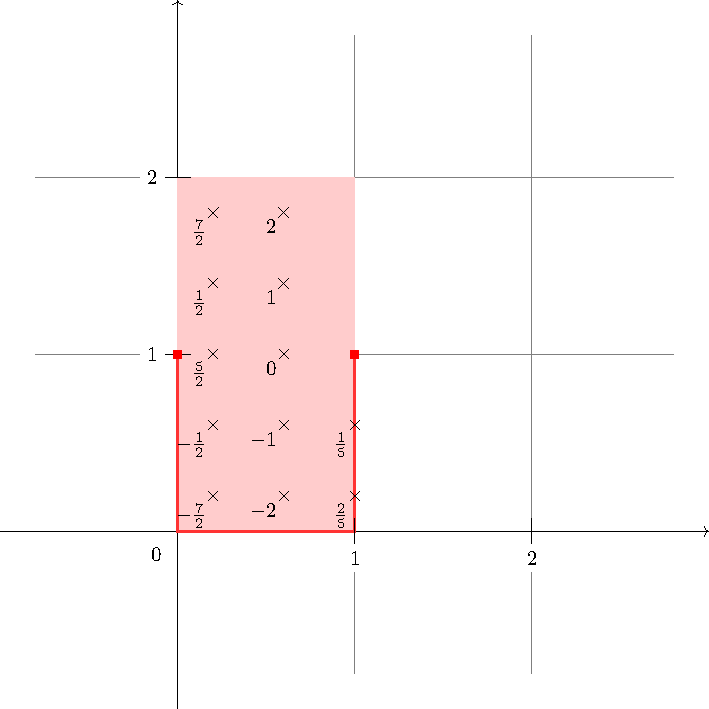
\includegraphics[scale=0.8]{pic/cuspofX(5).pdf}
		\caption{$X_0(5)$}
		\label{pic:cusps}
	\end{figure}
\end{example1}
\begin{theorem}[{\cite[Chapter 2, Lemma 2.7]{farkas2001theta}}]\
	\begin{enumerate}[1.]
		\item $\gamma \in \Gamma(N)$固定$X_0(N)$中的每个点.
		\item 设$\gamma \in \Gamma(1)$固定$X_0(N)$中的每个点,则$\gamma \in \pm\Gamma(N)$.
		%		\item 记$\Perm(X_0(N))$为$X_0(N)$的置换群,我们有群嵌入\vspace{-0.6cm}
		%		$$PSL_2(\mathbb{Z}/N\mathbb{Z}) \cong SL_2(\mathbb{Z})/\pm\Gamma(N) \hookrightarrow \Perm(X_0(N))$$\\[-1.8cm]
		%		$\,$
		\item 记$\Perm(X_0(N))$为$X_0(N)$的置换群,我们有群嵌入
		$$PSL_2(\mathbb{Z}/N\mathbb{Z}) \cong SL_2(\mathbb{Z})/\pm\Gamma(N) \hookrightarrow \Perm(X_0(N))$$
		\item 设$N>1$,则对每个$\chi \in X_0(N)$, $\theta[\chi]:=\theta[\chi](0,-)$为权$1/2$,特征为$\bigchi$的模形式,其中$\bigchi^{8k} \equiv 1 $.
	\end{enumerate}
	
\end{theorem}
\begin{proof}\
	\begin{enumerate}[1.]
		\item 回顾尖点的定义是$\mathbb{Q}^*/\Gamma(N)$.当然也可以通过计算验证.
		\item 记
		$$\chi_1(N):= \character{1}{\alpha/N} \qquad \chi_2(N):= \character{\alpha/N}{1} \qquad \chi_3(N):= \character{\alpha/N}{\alpha/N}$$
		其中
		$$\alpha=\begin{cases}
		0, & k=2\\
		1, & k\equiv 1 \;(\hspace{-4.2mm}\mod 2)\\
		2, & k\equiv 0 \;(\hspace{-3.8mm}\mod 4)\\
		4, & \text{其他}
		\end{cases}$$
		则$\chi_i(N) \in X_0(N)$,故$\gamma\chi_i(N)=\chi_i(N)$,从而算出$\gamma \in \pm\Gamma(N)$.
		\item 由1.与2.可知.
		\item 记$\chi:=\normalcharacter$, $\chi\gamma=\pm \chi +2nv_1+2n'v_2$,则
		$$\theta[\chi \gamma]=\exp \pi i \left\{ \epsilon n' \right\} \theta[\chi]$$
		代入\eqref{eq:Transformation3}得到
		\begin{equation}\label{eq:Transformation4}
		\theta[\chi](0,\gamma(\tau))=\kappa(\chi,\gamma) \exp \pi i \left\{ \epsilon n' \right\} \gamma'(\tau)^{-\frac{1}{4}} \theta[\chi] (0,\tau)
		\end{equation}
		记$\bigchi(\gamma)=\kappa(\chi,\gamma) \exp \pi i \left\{ \epsilon n' \right\}$,则$\theta[\chi]$为权$1/2$,特征为$\bigchi$的模形式.
	\end{enumerate}
	
\end{proof}

既然给出了模形式的例子,我们自然要关心其在尖点附近的性质.
\begin{defn}
	设$f$是$\mathcal{H}^*:=\mathcal{H} \cup \mathbb{R}^*$的函数, $\xi$为$X(\Gamma(k))$在$z \in \mathbb{R}^*$处的局部坐标,且有展开
	$$f(\tau)= \sum_{x \in \mathbb{R}}a_x\xi^x \qquad \{x \in \mathbb{R} \mid a_x \neq 0  \}\text{ 离散}$$
	则定义$f$在$z$点处的阶为
	$$\ord_zf(\tau):= \inf\{x \in \mathbb{R}\}a_x\xi^x \qquad \{x \in \mathbb{R} \mid a_x \neq 0\}.$$
\end{defn}

取正整数$k>1$,设$\chi=\character{m/k}{m'/k} \in X_0(k)$且$\chi$落在基本集中,注意$X(\Gamma(k))$在$\infty$处附近的局部坐标为$\xi:=\exp 2\pi i \tau/k$,且我们可以将$\theta[\chi]$表达成$\xi$的级数(这可视为$\theta$-级数在$\infty$处的展开),例如
$$\theta\character{m/k}{m'/k}=\xi^{\frac{m^2}{8k}} \sum_{n \in \mathbb{Z}} \exp \pi i \left\{ \frac{mm'}{2k}+\frac{m'n}{k} \right\} \xi ^{\frac{k}{2} n\left(n+\frac{m}{k} \right)}$$
故$\ord_{\infty} \theta[\chi]= \frac{m^2}{8k}$.类似地,我们得到
\begin{equation*}
\begin{aligned}
\ord_{\infty} \theta'[\chi]=& \begin{cases}
\frac{m^2}{8k}, & m \neq 0\\
\frac{k}{2}, & m=0
\end{cases} & \chi \neq \{v_1,v_2,v_3\} \\
\ord_{\infty} \frac{\theta'[\chi]}{\theta[\chi]}=& \begin{cases}
0, & m = 0 \text{ or }k,\; m'<k \\
\frac{k}{2}, & 0<m<k
\end{cases} & \chi \neq X(2) \\
\ord_{\gamma(x)} \theta[\chi](\tau)=&\;\ord_{x} \theta[\chi](\gamma\tau)=\ord_{x} \theta[\chi\gamma](\tau)\\
\ord_{\gamma(x)} \theta'[\chi](\tau)=&\;\ord_{x} \theta'[\chi](\gamma\tau)=\ord_{x} \theta'[\chi\gamma](\tau)\\
\end{aligned}
\end{equation*}


\subsection{$Y(\Gamma(N))$:全纯函数与射影嵌入}

为了具体给出空间$X(\Gamma(N))$上的亚纯函数,乃至于给出$X(\Gamma(N))$的射影嵌入,我们需要两个(或多个)同权同特征的模形式,以下为方便起见,设$N=k$为奇素数\footnote{读者可时刻取$k=5$或$k=7$作为例子,这也是我们故事的终点(不过这显然不是该数学领域的终点).}对$l=0,\ldots,\frac{k-3}{2}$,取$\chi_l:= \character{\frac{2l+1}{k}}{1} \in X_0(k)$,定义全纯函数
$$\varphi_l: \mathcal{H} \longrightarrow \mathbb{C} \qquad \tau \longmapsto \theta[\chi_l](0,k\tau)$$
\begin{theorem}[{\cite[p218]{farkas2001theta}}]
	函数$\varphi_l$ ($l=0,\ldots,\frac{k-3}{2}$)为级$\Gamma(k)$权$1/2$的模形式,且具有相同特征$\bigchi_k$.
\end{theorem}
\begin{proof}
	设
	$$\gamma = \begin{pmatrix}
	a & b \\ c & d
	\end{pmatrix}= \begin{pmatrix}
	a'k+1 & b'k \\ c'k & d'k+1
	\end{pmatrix}\in \Gamma(k), \qquad \hat{\gamma}:=\begin{pmatrix}
	a & bk \\ c/k & d
	\end{pmatrix},$$
	$$\chi_l=\character{t_l}{1}=\character{\frac{2l+1}{k}}{1}, \qquad \chi_l \hat{\gamma} := \chi_l+n_le_1+n_l'e_2,$$
	则有
	\begin{equation*}
	\begin{aligned}
	&\gamma'(\tau)^{\frac{1}{4}}\theta[\chi_l](0,k\gamma(\tau ))\hspace{3mm}\\
	=\hspace{3mm}& \hat{\gamma}'(k\tau)^{\frac{1}{4}}\theta[\chi_l](0,\hat{\gamma}(k\tau ))\\
	\xeq[]{\eqref{eq:Transformation4}}\;& \kappa(\chi_l, \hat{\gamma})\exp \pi i \{ t_ln_l' \} \theta[\chi_l](0,k\tau)		\\
	\end{aligned}
	\end{equation*}
	记$\bigchi_{k,l}(\gamma):=\kappa(\chi, \hat{\gamma})\exp \pi i \{ t_ln_l' \}$,则$\varphi_l$为级$\Gamma(k)$,特征$\bigchi_{k,l}(\gamma)$的模形式.接下来,我们只需计算$n_l'$并证明$\bigchi_{k,l}(\gamma)=\bigchi_{k,l'}(\gamma)$即可.
	
	由于
	$$\chi_l\hat{\gamma}=\character{at_l+\frac{c}{k}-a\frac{c}{k}}{bkt_l+d+bdk}=\character{t_l}{1}+\character{(a-1)t_l+\frac{c}{k}-a\frac{c}{k}}{bkt_l+d+bdk-1}$$
	可验证$(a-1)t_l+\frac{c}{k}-a\frac{c}{k}$, $bkt_l+d+bdk-1 \in 2\mathbb{Z}$,故$n_l'=\frac{1}{2}(bkt_l+d+bdk-1)$,此时
	\begin{equation*}
	\begin{aligned}
	\bigchi_{k,l}(\gamma)=\;& \exp 2\pi i \frac{1}{4} \left\{ -(at_l+\frac{c}{k})bdk-\frac{1}{2} \left( abkt_l^2+\frac{c}{k}d+2bct_l \right) \right\}\\
	& \cdot \exp 2\pi i \frac{1}{4} \left\{ t_l(bkt_l+d+bdk-1)  \right\}\\
	=\;& \exp 2\pi i \frac{1}{4} \left\{ (bk-\frac{1}{2}abk)t_l^2 +(d+bdk-1-abdk-bc)t_l-bcd-\frac{cd}{2k} \right\}
	\end{aligned}
	\end{equation*}
	故只需说明
	\begin{equation*}
	\begin{aligned}
	\frac{1}{4}t_l^2 (bk-\frac{1}{2}abk) \equiv\;&\frac{1}{4}t_{l'}^2 (bk-\frac{1}{2}abk) &(\hspace{-4.3mm}\mod \mathbb{Z})\\
	\frac{1}{4}t_l(d+bdk-1-abdk-bc) \equiv\;& \frac{1}{4}t_{l'}(d+bdk-1-abdk-bc)  &(\hspace{-4.3mm}\mod \mathbb{Z})
	\end{aligned}
	\end{equation*}
	即可,这等价于证明
	\begin{equation*}
	\begin{aligned}
	&(l-l')(l+l'+1)(b'-\frac{1}{2}ab') \in \mathbb{Z}\\
	&\frac{1}{2}(l-l')(d'+bd-abd-b'c'k) \in \mathbb{Z}
	\end{aligned}
	\end{equation*}
	由初等数论知识\footnote{例如, $d'+bd-abd-b'c'k \equiv (d+1) +bd+abd+bc \equiv d+bd+abd+ad \equiv d(a+1)(b+1) \equiv 0 \;\;(\hspace{-2.4mm}\mod 2)$.}可知成立.
\end{proof}
\begin{corollary}
	$\varphi_l/\varphi_{l'}$为$\mathcal{H}/\Gamma(k)$上无零点的全纯函数,且我们有良定的全纯映照
	$$\Phi: \mathcal{H}/\Gamma(k) \longrightarrow \mathbb{PC}^{\frac{k-3}{2}} \qquad \bar{\tau} \longmapsto \left[ \varphi_0(\tau),\ldots , \varphi_{\frac{k-3}{2}}(\tau) \right]$$
\end{corollary}

在接下来的篇幅中,我们将
\begin{itemize}
	\item 延拓$\varphi_l/\varphi_{l'}$至$X(\Gamma(k))$上的亚纯函数并计算其除子;
	\item 延拓$\Phi$至$X(\Gamma(k))$;
	\item 描述$\Gamma(1)$在$\Img \Phi$中的作用(以$\frac{k-1}{2} \times \frac{k-1}{2}$的矩阵表达!),并利用$\Gamma(1)$在尖点集合作用的可递性来找出尖点的像;
	\item 对$k=5,7$,证明$\Phi$为嵌入映射\footnote{然而我不知道一般情况是否如此,书中认为是一个猜想.};
\end{itemize}
\subsection{$X(\Gamma(N))$:尖点与亚纯函数}
为了更方便地观察尖点的性质,我们通过映射
$$\Psi: \mathbb{Q}^*/\Gamma(k) \longrightarrow \mathbb{Q}^*/\Gamma_0(k)$$
将尖点分成两类,其中
$$\Gamma_0(k):=\left\{ \begin{pmatrix}
a &b \\ c & d
\end{pmatrix} \in SL_2(\mathbb{Z}) \;\middle|\; \begin{pmatrix}
a &b \\ c & d
\end{pmatrix} \equiv \begin{pmatrix}
* & * \\ 0 & *
\end{pmatrix} \mod k  \right\}$$
对偶地定义
$$\Gamma^0(k):=\left\{ \begin{pmatrix}
a & b \\ c & d
\end{pmatrix} \in SL_2(\mathbb{Z}) \;\middle|\; \begin{pmatrix}
a & b \\ c & d
\end{pmatrix} \equiv \begin{pmatrix}
* & 0 \\ * & *
\end{pmatrix} \mod k  \right\}$$
注意到这两个同余子群之间的共轭同构:
$$\Gamma_0(k) \longrightarrow \Gamma^0(k) \qquad \begin{pmatrix}
a & b \\ c & d
\end{pmatrix} \longmapsto \begin{pmatrix}
a & bk \\ c/k & d
\end{pmatrix}$$
\begin{lemma}\
	\begin{enumerate}[(1)]
		\item $\mathbb{Q}^*/\Gamma_0(k)=\{\bar{\infty}, \bar{0} \}$.换句话说,对任意$r \in \mathbb{Q}^*$,存在$\gamma \in \Gamma_0(k)$,使得$\gamma (0)=r$或$\gamma (\infty)=r$;
		\item $$\Psi^{-1}(\bar{\infty})= \left\{ \Gamma(k) \frac{2l+1}{k} \;\middle|\; l=0,\ldots,\frac{k-3}{2} \right\}$$
		\item 对$\gamma=\left(\begin{smallmatrix}
		a & b \\ c & d
		\end{smallmatrix}\right) \in \Gamma_0(k)$,记$\hat{\gamma}\left(\begin{smallmatrix}
		a & bk \\ c/k & d
		\end{smallmatrix}\right)$,则存在置换$\sigma_{\gamma} \in \Perm \{0,\ldots,\frac{k-3}{2} \}$与特征$\tilde{\kappa}(\chi_l,-):\Gamma^0(k) \longrightarrow \mathbb{C}^*$,使得
		$$\gamma^{\frac{1}{4}}(\tau)\varphi_l(\gamma\tau)=\tilde{\kappa}(\chi_l,\hat{\gamma})\varphi_{\sigma_{\gamma}(l)}(\tau) $$
	\end{enumerate}
	
\end{lemma}
\begin{proof}\
	\begin{enumerate}[(1)]
		\item 记$\gamma=\left(\begin{smallmatrix}
		a & b \\ c'k & d
		\end{smallmatrix}\right)$,则$\gamma (0)=\frac{b}{d}$, $\gamma (\infty)=\frac{a}{c'k}$;另一方面,对任意$r \in \mathbb{Q}^*$,记$r=\frac{x}{y}$, $x,y$互质\footnote{当$r=\infty$时,形式上记$r=\frac{1}{0}$.}.
		\begin{itemize}
			\item 当$k \nmid y$时,存在$a,c' \in \mathbb{Z}$使得$ay-c'kx=1$,取$\gamma:=\left(\begin{smallmatrix}
			a & x \\ c'k & y
			\end{smallmatrix}\right)$,则$\gamma(0)=r$;
			\item 当$k \mid y$时,存在$b,d \in \mathbb{Z}$使得$xd-by=1$,取$\gamma:=\left(\begin{smallmatrix}
			x & b \\ y & d
			\end{smallmatrix}\right)$,则$\gamma(\infty)=r$.
		\end{itemize}
		\item 注意到同构\eqref{eq:cusppointiso}.
		\item $\chi_l \hat{\gamma}$一定可以写为$\pm \chi_{\sigma_{\gamma}(l)}+n_le_1+n_l'e_2$的形式,而
		\begin{equation*}
		\begin{aligned}
		&\gamma'(\tau)^{\frac{1}{4}}\theta[\chi_l](0,k\gamma(\tau ))\hspace{3mm}\\
		=\hspace{3mm}& \hat{\gamma}'(k\tau)^{\frac{1}{4}}\theta[\chi_l](0,\hat{\gamma}(k\tau ))\\
		\xeq[]{\eqref{eq:Transformation4}}\;& \kappa(\chi_l, \hat{\gamma})\exp \pi i \left\{ \frac{(2l+1)}{k}n_l' \right\} \theta[\chi_l](0,k\tau)		\\
		\end{aligned}
		\end{equation*}
	\end{enumerate}
\end{proof}
\begin{example1}\label{example:Gamma5}
	当$k=5$时, $\displaystyle\Psi^{-1}(\bar{\infty})=\left\{\Gamma(5)\frac{1}{5},\,\Gamma(5)\frac{3}{5} \right \}$,
	$$\frac{1}{5}= \begin{pmatrix}
	1 & 0 \\ 5 & 1
	\end{pmatrix}\infty \qquad \frac{3}{5}= \begin{pmatrix}
	3 & 1 \\ 5 & 2
	\end{pmatrix}\infty$$
	$$\character{1/5}{1} \begin{pmatrix}
	1 & 0 \\ 1 & 1
	\end{pmatrix} =\character{1/5}{1} \qquad 
	\character{3/5}{1} \begin{pmatrix}
	1 & 0 \\ 1 & 1
	\end{pmatrix} =\character{3/5}{1}$$
	故$\sigma_{\left[\begin{smallmatrix}
		1 & 0 \\ 5 & 1
		\end{smallmatrix}\right]} (0)=0$, $\sigma_{\left[\begin{smallmatrix}
		1 & 0 \\ 5 & 1
		\end{smallmatrix}\right]} (1)=1$,
	$\sigma_{\left[\begin{smallmatrix}
		1 & 0 \\ 5 & 1
		\end{smallmatrix}\right]} =\Id_{\{0,1\}}$.
	$$\character{1/5}{1} \begin{pmatrix}
	3 & 5 \\ 1 & 2
	\end{pmatrix} \equiv\character{3/5}{1} \qquad 
	\character{3/5}{1} \begin{pmatrix}
	3 & 5 \\ 1 & 2
	\end{pmatrix} \equiv\character{1/5}{1}$$ 	
	故$\sigma_{\left[\begin{smallmatrix}
		3 & 1 \\ 5 & 2
		\end{smallmatrix}\right]} (0)=1$, $\sigma_{\left[\begin{smallmatrix}
		3 & 1 \\ 5 & 2
		\end{smallmatrix}\right]} (1)=0$,
	$\sigma_{\left[\begin{smallmatrix}
		3 & 1 \\ 5 & 2
		\end{smallmatrix}\right]} =(01)$.
\end{example1}
\begin{example1}
	当$k=7$时, $\displaystyle\Psi^{-1}(\bar{\infty})=\left\{\Gamma(7)\frac{1}{7},\,\Gamma(7)\frac{3}{7},\,\Gamma(7)\frac{5}{7} \right \}$,
	$$\frac{1}{7}= \begin{pmatrix}
	1 & 0 \\ 7 & 1
	\end{pmatrix}\infty \qquad \frac{3}{7}= \begin{pmatrix}
	3 & 2 \\ 7 & 5
	\end{pmatrix}\infty \qquad \frac{5}{7}= \begin{pmatrix}
	5 & 2 \\ 7 & 3
	\end{pmatrix}\infty$$
	计算得到$\sigma_{\left[\begin{smallmatrix}
		1 & 0 \\ 7 & 1
		\end{smallmatrix}\right]} =\Id_{\{0,1,2\}}$ , $\sigma_{\left[\begin{smallmatrix}
		3 & 2 \\ 7 & 5
		\end{smallmatrix}\right]} =(012)$, $\sigma_{\left[\begin{smallmatrix}
		5 & 2 \\ 7 & 3
		\end{smallmatrix}\right]} =(021)$.
\end{example1}

\begin{theorem}[{\cite[Chapter 3, Lemma 5.1]{farkas2001theta}}]
	设$x \in \mathbb{Q}$, $\gamma \in \Gamma_0(k)$, $\gamma (\infty)=r$或$\gamma(0)=r$, $l \in \left\{ 0,\ldots,\frac{k-3}{2} \right\}$.
	\begin{enumerate}[(1)]
		\item 若$\gamma(\infty)=r$,则$\ord_r \varphi_l=\frac{1}{8}(2\sigma_{\gamma}(l)+1)^2$.
		\item 若$\gamma(0)=r$,则$\ord_r \varphi_l=\frac{1}{8}$.
	\end{enumerate}
\end{theorem}
\begin{proof}\
	\begin{enumerate}[(1)]
		\item $\ord_r \varphi_l=\ord_{\infty} \varphi_{\sigma_{\gamma}(l)}=\frac{1}{8}(2\sigma_{\gamma}(l)+1)^2$.
		\item 取$A:= \left(\begin{smallmatrix}
		0 & 1 \\ -1 & 0
		\end{smallmatrix} \right)$,则
		\begin{equation*}
		\begin{aligned}
		&\ord_0 \varphi_l=\ord_{A(\infty)} \character{t_l}{1}(0,k\tau)=\ord_{\infty} \character{t_l}{1}(0,kA\tau)\\
		=\;&\ord_{\infty} \character{1}{t_l}(0,\tau/k)=\frac{1}{k} \cdot \frac{k^2}{8k}= \frac{1}{8}.
		\end{aligned}
		\end{equation*}
	\end{enumerate}
\end{proof}

\begin{example1}
	当$k=5$时,直接将例 \ref{example:Gamma5}的结论代入得
	$$\ord_{\frac{1}{5}}\varphi_0= \frac{1}{8} \left(  2\sigma_{\left[\begin{smallmatrix}
		1 & 0 \\ 5 & 1
		\end{smallmatrix}\right]} (0)+1 \right)^2=\frac{1}{8} \qquad \ord_{\frac{3}{5}}\varphi_0= \frac{9}{8}$$
	借助黎曼面中除子的概念,记
	$$\divi \varphi_0:= \frac{1}{8}P_{\frac{1}{5}}+\frac{9}{8}P_{\frac{3}{5}}+\frac{1}{8} \sum_{r \sim 0}P_r,$$
	同理可得
	$$\divi \varphi_1= \frac{9}{8}P_{\frac{1}{5}}+\frac{1}{8}P_{\frac{3}{5}}+\frac{1}{8} \sum_{r \sim 0}P_r.$$
\end{example1}
\begin{example1}
	当$k=7$时,经计算得
	$$\divi \varphi_0= \frac{1}{8}P_{\frac{1}{7}}+\frac{9}{8}P_{\frac{3}{7}}+\frac{25}{8}P_{\frac{5}{7}}+\frac{1}{8} \sum_{r \sim 0}P_r.$$
	$$\divi \varphi_1= \frac{9}{8}P_{\frac{1}{7}}+\frac{25}{8}P_{\frac{3}{7}}+\frac{1}{8}P_{\frac{5}{7}}+\frac{1}{8} \sum_{r \sim 0}P_r.$$
	$$\divi \varphi_2= \frac{25}{8}P_{\frac{1}{7}}+\frac{1}{8}P_{\frac{3}{7}}+\frac{25}{8}P_{\frac{5}{7}}+\frac{9}{8} \sum_{r \sim 0}P_r.$$
\end{example1}
\begin{corollary}\
	\begin{enumerate}[(1)]
		\item $\varphi_l/\varphi_l'$为$X(\Gamma(k))$上的亚纯函数,在$\gamma(0)$上的阶为($\gamma \in \Gamma_0(k)$)
		$$\ord_{\gamma(0)} \varphi_l/\varphi_{l'} = \frac{1}{2} (\sigma_{\gamma}(l)-\sigma_{\gamma}(l'))(\sigma_{\gamma}(l)+\sigma_{\gamma}(l')+1)$$
		\item $\Phi$可延拓至$X(\Gamma(N))$.
	\end{enumerate}
	
\end{corollary}
%按照流程,接下来我们将刻画$\Gamma(1)$在$\Img \Phi$中的作用。
\subsection{$\Img \Phi$上的群作用}
令$V(k):=\left<\phi_l \;\middle|\; l=0,\ldots,\frac{k-3}{2}  \right>$,可以验证$\phi_0,\ldots, \phi_{\frac{k-3}{2}}$线性无关,故$V(k)$为$\frac{k-1}{2}$维$\mathbb{C}$-线性空间。对$\gamma \in \Gamma(1)$,定义$\gamma$在$V(k)$上的作用
$$\gamma_*\colon V(k) \longrightarrow V(k) \qquad \left[\gamma_* (\varphi_l) \right](\tau):=\big((\gamma^{-1})'(\tau)\big)^{\frac{1}{4}} \,\cdot \,\varphi_l(\gamma^{-1}\tau)$$
\begin{theorem}[{\cite[Chapter 3, Lemma 4.2]{farkas2001theta}}]\
	\begin{enumerate}[(1)]
		\item 该定义为良定的$\mathbb{C}$-线性映射,且有群作用
		\begin{equation}\label{eq:groupactionondual}
		\Gamma(1) \times V(k) \longrightarrow V(k) \qquad (\gamma_*,\varphi) \longmapsto \gamma_*(\varphi)
		\end{equation}
		\item 群作用\eqref{eq:groupactionondual}诱导$\Gamma(1)$在$\mathbb{PC}^{\frac{k-3}{2}} \cong \mathbb{P}V^{\vee}(k)$上的作用,且全纯映照
		$$\Phi: \mathcal{H}/\Gamma(k) \longrightarrow \mathbb{P}V^{\vee}(k) \qquad \bar{\tau} \longmapsto \left[ \varphi_0(\tau),\ldots , \varphi_{\frac{k-3}{2}}(\tau) \right]$$
		为$\Gamma(1)$-等变映射。
	\end{enumerate}
	
\end{theorem}
\begin{proof}\
	\begin{enumerate}[(1)]
		\item 容易得到$\gamma_*s_*=(\gamma s)_*$,故只需证明该结论对$\Gamma(1)$的生成元
		$$A:=\begin{pmatrix}
		0 & 1 \\ -1 & 0
		\end{pmatrix}\qquad B:=\begin{pmatrix}
		1 & 1 \\ 0 & 1
		\end{pmatrix}$$
		成立即可。
		\begin{equation*}
		\begin{aligned}
		\left[A_*(\varphi_l) \right](\tau) =\;& \big((A^{-1})'(\tau)\big)^{\frac{1}{4}}  \theta [\chi_l](0,-\frac{k}{\tau})\\
		=\;& \exp \left\{ \frac{\pi i}{2} \right\} \kappa (\chi_l,A) \theta \character{1}{t_l}(0,\frac{\tau}{k})\\
		=\;& \exp \left\{ \frac{\pi i}{2} \right\} \kappa (\chi_l,A)\sum_{l'=0}^{k-1} \theta\character{\frac{1+2l'}{k}}{kt_v}(0,k\tau)\\
		=\;& \exp \left\{ \frac{\pi i}{2} \right\} \kappa (\chi_l,A)\sum_{l'=0}^{k-1} \exp \left\{ \pi i t_l l \right\} \varphi_{l'}(\tau)
		\end{aligned}
		\end{equation*}
		\begin{equation*}
		\begin{aligned}
		\left[B_*(\varphi_l) \right](\tau) =\;& \theta[\chi_l] (0,k\tau-k)\\
		=\;& \kappa (\chi_l,B^{-k}) \theta\character{t_l}{-kt_l-k+1}(0,k\tau)\\
		=\;& \kappa (\chi_l,B^{-k}) \exp -\frac{\pi i}{2}  \left\{ t_l(2l+k+1) \right\} \varphi_{l'}(\tau)
		\end{aligned}
		\end{equation*}
		\item 直接验证下列图表的交换性:
		\begin{center}
			
			\begin{tikzcd}
				\tau \arrow[d, "\gamma"] \arrow[r, hook] & V^{\vee}(k) \arrow[d, "\gamma_*^{\vee}", dashed] \arrow[r, dashed] & \mathbb{P}V^{\vee}(k) \arrow[d, "\gamma_*^{\vee}"] \\
				\gamma\tau \arrow[r, hook]               & V^{\vee}(k) \arrow[r, dashed]                                      & \mathbb{P}V^{\vee}(k)                             
			\end{tikzcd}
		\end{center}
	\end{enumerate}
	
	
\end{proof}
\begin{remark}
	通过更细致的计算可以得到线性映射的系数,这里我们只给出$k=5$,取$\phi_0,\phi_l$为单位正交基时的情况:
	$$A_*=\sqrt{\frac{i}{5}} \begin{pmatrix}
	-\omega_{20}^9-\omega_{20}^{-9} & \omega_{20}+\omega_{20}^{-5} \\ \omega_{20}^5+\omega_{20}^{-1} & -\omega_{20}-\omega_{20}^{-1}
	\end{pmatrix} \qquad B_*= \exp \left\{-\frac{\pi i}{20} \right\}\begin{pmatrix}
	1 & 0\\ 0 & \omega_5^{-1}
	\end{pmatrix}$$
	将其视作分式线性变换时,其恰好生成群$\Gamma_{(2,3,5)}$!
\end{remark}
另外,我们还可以在$V(k)$上定义良定的内积结构:
$$\left< \varphi, \psi \right> := \int_{\mathcal{H}/\Gamma(k) } \left( \Img z \right)^{-\frac{3}{2}} \varphi(z) \overline{\psi(z)} \,\left|dz\overline{dz}\right|$$
接下来的定理解释了为什么$\varphi_0,\ldots,\varphi_{\frac{k-3}{2}}$如此特殊:它们相互正交!
\begin{theorem}[{\cite[Chapter 3, Proposition 4.8]{farkas2001theta}}]\
	\begin{enumerate}[(1)]
		\item 对$\gamma \in \Gamma$, $\gamma_*$为酉变换,对应的矩阵为酉方阵;
		\item 向量组$\left\{ \varphi_0,\ldots,\varphi_{\frac{k-3}{2}}  \right\}$为$V(k)$的一组正交基,且具有相同的范数.
	\end{enumerate}
	
\end{theorem}
\begin{proof}\
	\begin{enumerate}[(1)]
		\item 我们有
		\begin{equation*}
		\begin{aligned}
		\left< \gamma_*\varphi, \gamma_*\psi \right>=\;&\int_{\mathcal{H}/\Gamma(k) } \left( \Img z \right)^{-\frac{3}{2}} \left(\gamma'(z)\right)^{-\frac{1}{2}}\varphi(\gamma^{-1}z) \overline{\psi(\gamma^{-1}z)} \,\left|dz\overline{dz}\right|\\
		=\;&\int_{\mathcal{H}/\Gamma(k) } \left( \Img \gamma^{-1}z \right)^{-\frac{3}{2}} \varphi(\gamma^{-1}z) \overline{\psi(\gamma^{-1}z)} \,\left|d(\gamma^{-1}z)\overline{d(\gamma^{-1}z)}\right|\\
		=\;& \left< \varphi, \psi \right>
		\end{aligned}
		\end{equation*}
		\item $\phi_l$为$B_*$对应特征值$\lambda_l:=c(B,k)\exp \left\{ \frac{\pi i}{k}(l^2+l) \right\}$的特征向量,而对于酉变换,不同特征值空间两两正交。至于相同的特征值,取$\gamma \in \Gamma(1)$使得$\gamma_*(\varphi_l)=\bigchi\varphi_{l'}$,则
		$$\left< \varphi_{l'}, \varphi_{l'} \right>=\left< \bigchi\varphi_{l'}, \bigchi\varphi_{l'} \right>=\left< \gamma_*(\varphi_{l}, \gamma_*(\varphi_{l}) \right>=\left< \varphi_{l}, \varphi_{l} \right>$$
	\end{enumerate}
\end{proof}
\section{应用:正二十面体群与Klein四次曲线}
本节分别讨论$k=5$与$k=7$的情况,部分信息已经作为例子包含于第\ref{sec:consofmodularform}小节。

\begin{theorem}
	$j$在复乘点取代数数。可以算出$j(i)=1728$, $j(\omega_3)=0$.
\end{theorem}
\begin{proof}
	这是复乘理论的基本内容,参见\cite[6.1]{zagier1984series}.
\end{proof}
\subsection{$k=5$, $j_5$-函数}
定义$j_5(\tau):=\omega_5^{-1} \frac{\varphi_1(\tau)}{\varphi_0(\tau)}$, $\hat{j}_5:X(\Gamma(5)) \longrightarrow \mathbb{PC}^1$由$j_5$诱导,则
\begin{enumerate}[(1)]
	\item $\hat{j}_5$为$X(\Gamma(5))$上的亚纯函数, $\divi \hat{j}_5 =P_{\frac{1}{5}}-P_{\frac{3}{5}}$.
	\item 取
	$$S:= \begin{pmatrix}
	\omega_5^3 & 0\\ 0 & \omega_5^2
	\end{pmatrix} \qquad T=\frac{1}{\sqrt{5}}\begin{pmatrix}
	\omega_5-\omega_5^4 & \omega_5^3-\omega_5^2 \\
	\omega_5^3-\omega_5^2 & \omega_5^4-\omega_5
	\end{pmatrix}$$
	则
	\begin{equation}\label{eq:j5trans}
	j_5 (\tau+1)=S j_5 (\tau)=\omega_5 j_5 (\tau) \qquad j_5 (-\frac{1}{\tau})=T j_5 (\tau)
	\end{equation}
	\item 通过\eqref{eq:j5trans}得到$j_5 (i) \in \{t_+,t_- \}$, $j_5 (\omega_5) \in \{\omega_+,\omega_- \}$,其中
	$$t_{\pm}= -\frac{\sqrt{5}+1}{2} \pm \sqrt{\frac{5+\sqrt{5}}{2}} \qquad \omega_{\pm}=\omega_5^2 \frac{3+\sqrt{5}\pm \sqrt{30+6\sqrt{5}}}{4} .$$
	\item $\hat{j}_5$给出了$X(\Gamma(5))$ 至 $\mathbb{PC}^1$的黎曼面同构,将$\Gamma(1)\infty$映至正十二面体的12个面心顶点上,将$\Gamma(1)i$映至边点,将$\Gamma(1)\omega_3$映至顶点上。
	\item 记$I:= \hat{j} \circ \pi_1 \circ \hat{j}_5^{-1}$, $G:=\left< S,T  \right>$,观察图表
	\begin{figure}[ht]
		
		\begin{minipage}[t]{.3\textwidth}
			\begin{tikzcd}
				\mathcal{H}^*/\Gamma(5) \arrow[r, "\pi_1"] \arrow[d, "\hat{j}_5","\sim"'] & \mathcal{H}^*/\Gamma(1) \arrow[d, "\hat{j}","\sim"'] \\
				\mathbb{PC}^1 \arrow[r, "I"]                                      & \mathbb{PC}^1                               
			\end{tikzcd}
		\end{minipage}
		\hspace{.04\textwidth}
		\begin{minipage}[t]{.6\textwidth}
			\begin{tikzcd}[column sep=small]
				\Gamma(1)i \arrow[d, maps to] \arrow[r, maps to] & i \arrow[d, maps to] & \Gamma(1)\omega_3 \arrow[r, maps to] \arrow[d, maps to] & \omega_3 \arrow[d, maps to] & \Gamma(1)\infty \arrow[d, maps to] \arrow[r, maps to] & \infty \arrow[d, maps to] \\
				Gt_{\pm} \arrow[r, maps to]                      & 1728                    & G\omega_{\pm} \arrow[r, maps to]                        & 0                           & G\infty \arrow[r, maps to]                            & \infty                   
			\end{tikzcd}
		\end{minipage}
	\end{figure}
	故$I/Z_5$为$\mathbb{PC}^1$上的全纯函数,故为常值,计算后得到$I=1728Z_5$,这样我们解决了上一章末尾留下的任务。
\end{enumerate}
\begin{remark}\
	\begin{enumerate}[1.]
		\item 事实上可以算出$j_5 (i)= t_+$, $j_5 (\omega_5)=\omega_+$.
		\item $j_5$有多种多样的表达方式。例如,
		\begin{equation*}
		\begin{aligned}
		j_5(\tau)=\;& \omega_5^{-1}\frac{\theta \character{3/5}{1}(0,5\tau)}{\theta \character{1/5}{1}(0,5\tau)}=q^{\frac{1}{5}} \frac{\theta_{00}(3\tau,5\tau)}{\theta_{00}(\tau,5\tau)}\\
		=\;& q^{\frac{1}{5}}\frac{\displaystyle \sum_{n \in \mathbb{Z}}q^{\frac{5n^2+3n}{2}}}{\displaystyle \sum_{n \in \mathbb{Z}}q^{\frac{5n^2+n}{2}}}=q^{\frac{1}{5}} \prod_{n \geqslant 1}(1-q^n)^{\left(\frac{n}{5}\right)} 
		\end{aligned}
		\end{equation*}
		其中$\left(\frac{n}{5} \right)$为Kronecker符号\footnote{$$\left(\frac{n}{5} \right)=\begin{cases}
			0, & n \equiv 0\phantom{,1}\;(\hspace{-3.4mm}\mod 5)\\
			1, & n \equiv 1,4 \;(\hspace{-3.4mm}\mod 5)\\
			-1, & n \equiv 2,3 \;(\hspace{-3.4mm}\mod 5)\\
			\end{cases}$$}.此外,$j_5$还有连分数表示:
		$$j_5(\tau)=\frac{q^{\frac{1}{5}}}{\displaystyle 1+\frac{q}{\displaystyle 1+\frac{q^2}{1+\cdots}}}$$
		代入$\tau=0,i,\omega_3$可以得到不同的连分数恒等式。
	\end{enumerate}
\end{remark}
\subsection{$k=7$, Klein四次曲线}
由Riemann-Roch定理,映射$\Phi$为射影嵌入\footnote{参见\cite[p246-247]{farkas2001theta}}。我们将导出$\Img \Phi$对应的方程。

记$$f_0=\frac{\varphi_1}{\varphi_2}, \qquad f_1=\frac{\varphi_2}{\varphi_0}, \qquad f_2=\frac{\varphi_0}{\varphi_1}$$
为三个$X(\Gamma(N))$上的亚纯函数,已知其除子分别为
\begin{equation*}
\begin{aligned}
\divi (f_0)=-2P_{\frac{1}{7}}+3P_{\frac{3}{7}}-P_{\frac{5}{7}},\\
\divi (f_1)=+3P_{\frac{1}{7}}-P_{\frac{3}{7}}-2P_{\frac{5}{7}},\\
\divi (f_2)=-P_{\frac{1}{7}}-2P_{\frac{3}{7}}+3P_{\frac{5}{7}},
\end{aligned}
\end{equation*}
配凑得
$$\divi(f_2/f_1^2)=-7P_{\frac{1}{7}}+7P_{\frac{5}{7}} \qquad \divi(f_0^2/f_1)=-7P_{\frac{1}{7}}+7P_{\frac{3}{7}}$$
故$f_2/f_1^2$与$f_0^2/f_1$之间相差一个仿射变换。解方程得到
$$\frac{f_2}{f_1^2}= \omega_7^{-1}\frac{f_0^2}{f_1}+\omega_7^2$$
亦即
$$\phi_2\phi_0^3=\omega_7^{-1}\phi_0\phi_1^3 +\omega_7^{2}\phi_1\phi_2^3$$
在线性变换
$$X=\omega_7^4\varphi_0, \qquad Y=\varphi_1, \qquad Z= \varphi_2,$$之后得到极其优美的方程$$X^3Y+Y^3Z+Z^3X=0.$$可以直接验证这个方程确定的曲面确实是亏格为$3$的光滑的黎曼面,并且具有丰富的对称性: $\Gamma(1)/\Gamma(7) \cong PSL_2(\mathbb{F}_7)$是它的自同构群,阶数为168.史称该曲线为Klein四次曲线。
\nocite{nash2014klein}\nocite{hilton1991catalan}\nocite{duke2005continued}
\nocite{green1978on}\nocite{klein1892vorlesungen}\nocite{fricke1897vorlesungen}\nocite{shimura1971introduction}\nocite{shurman1997geometry}\nocite{anvari2009automorphisms}\nocite{mumford1995algebraic}
%然后第三节写一下用$\theta$函数来构造主同余子群的模形式(显然!)将特征的等价类与尖点、$\pm \textbackslash(\mathbb{Z}/N\mathbb{Z})^2_{\prim}$联系起来,构造特殊的模形式.
%
%第四节写一下那三个特殊情况,要写下连分数
%
%举的例子是$\Gamma(2),\Gamma(5),\Gamma(7)$,这三个例子分别对应着$C-{0,1}$的万有覆叠(推出Picard定理),正二十面体群,Klein四次曲线
  %自行添加
  %\include{chapter/...}

%%%%%%%%%%%%%%%%%%%%%%%%%%%%%%
%% 附件部分
%%%%%%%%%%%%%%%%%%%%%%%%%%%%%%
\backmatter

\renewcommand\refname{{\textbf{参考文献}}}
\bibliography{reference}	
\bibliographystyle{ieeetr}


\end{document}
